\chapter{കേരളത്തിൽ റാണിമാർ ഉണ്ടായിരുന്നോ?}
\label{chapter3}
\begin{figure}[h]
\begin{center}
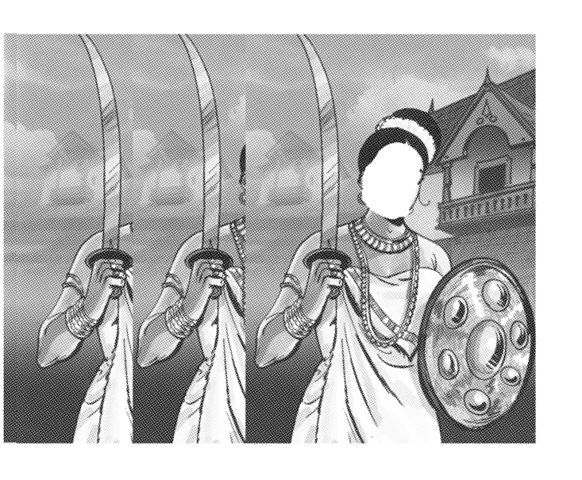
\includegraphics[width=\textwidth,height=7cm]{Kulasthree_Chapter_three_pic01.jpg}
\end{center}
%\caption*{പുലയർ - കെ പി പത്മനാഭ മേനോൻ - വാള്യം 3, (1929), 1984}
\end{figure}

\paragraph{}പഞ്ചായത്തുകളിലെ സ്ത്രീസംവരണം 33ൽനിന്ന് 50 ശതമാനമായി ഉയർന്നിരിക്കുന്ന ഇന്നത്തെക്കാലത്തും കേരളരാഷ്ട്രീയത്തിന്റെ ഉന്നതങ്ങളിൽ വളരെക്കുറച്ചു സ്ത്രീകളേയുള്ളു. എളിയ മട്ടിൽ ജനസേവനം നടത്തുന്ന സ്ത്രീകളോട് നമുക്കു വളരെ പ്രിയമാണ്. എന്നാൽ അധികാരരാഷ്ട്രീയത്തിൽ പ്രവേശിക്കാൻ ശ്രമിക്കുന്ന സ്ത്രീകളെ അല്പമൊരു പുച്ഛത്തോടെയാണ് നാം കാണുന്നത്. 'പൗരുഷക്കാരി,' 'തന്റേടി' മുതലായ വിശേഷണങ്ങളാണ് നാം അവർക്കു നൽകാറുള്ളത്! പുരുഷന്മാർക്ക് രാഷ്ട്രീയാധികാരത്തെ മൊത്തത്തിൽ തീറെഴുതിക്കൊടുക്കുന്ന ഈ രീതി എങ്ങനെയാണ് രൂപപ്പെട്ടത്? മലയാളികളുടെ പരമ്പരാഗത രാഷ്ട്രീയസ്ഥാപനങ്ങളിൽ - രാജസ്വരൂപങ്ങളിൽ - ആ സ്ഥാനങ്ങളിലെത്തിയ സ്ത്രീകൾക്ക് ചില സാദ്ധ്യതകളുണ്ടായിരുന്നുവെന്നും ക്രമേണ അവ നഷ്ടമാവുകയാണുണ്ടായതെന്നും നാം തിരിച്ചറിയേണ്ടതുണ്ട്.

\paragraph{}ആമുഖത്തിൽ പറഞ്ഞ കാര്യങ്ങളുടെ വെളിച്ചത്തിൽ ഈ ചോദ്യത്തിന് വലിയ പ്രാധാന്യം കൊടുക്കേണ്ടതില്ലെന്ന് നമുക്ക് വാദിക്കാവുന്നതാണ്. നമ്മുടെ ഭൂതകാലം ചികഞ്ഞുനോക്കിയാൽ ഒന്നോ രണ്ടോ കഴിവുറ്റ റാണിമാരെ കണ്ടെത്താൻ കഴിയും. പക്ഷേ, ആ കണ്ടെത്തലിൽനിന്ന് നമുക്കെന്താണു ഗുണം? നേരത്തേ പറഞ്ഞതുപോലെ, ഒരു ഉണ്ണിയാർച്ചയെ കണ്ടെത്തിയെന്നു കരുതി അന്നത്തെ ഇവിടത്തെ പെണ്ണുങ്ങൾ മുഴുവൻ കളരിപഠിച്ച അഭ്യാസികളായിരുന്നുവെന്ന് പറയാൻപറ്റുമോ? പറ്റില്ല, തീർച്ച! അതുപോലെ, ഒന്നുരണ്ട് നല്ല ഭരണാധികാരിണികളെ കണ്ടെത്തിയെന്നു കരുതി അന്നത്തെ മേലാളസ്ത്രീകൾക്ക് ഭരണാധികാരത്തിൽ പുരുഷനുതുല്യമായ നിലയുണ്ടായിരുന്നുവെന്ന് വാദിക്കാൻ കഴിയില്ല. ഒന്നാമത്, റാണിമാരെ സാധാരണസ്ത്രീകളുടെ കൂട്ടത്തിൽപെടുത്താൻപറ്റില്ല. അവർ ഉന്നതജാതിക്കാരും കുടുംബക്കാരുമായിരുന്നു. രണ്ടാമത്, ഒന്നുരണ്ടുദാഹരണങ്ങൾ തിരഞ്ഞുപിടിക്കുന്നതുകൊണ്ട് സ്ത്രീ പുരുഷനു തുല്യയായിരുന്നുവെന്ന് സമർത്ഥിക്കാനാവില്ല - ഏതു സമൂഹത്തിലും പുരുഷനൊപ്പം നിൽക്കുന്ന ഒന്നുരണ്ട് അസാമാന്യസ്ത്രീകൾ ഉണ്ടാകുമെന്ന മറുപടിയായിരിക്കും കിട്ടുക.
\paragraph{}എങ്കിലും പഴയ മലയാളിസമൂഹത്തിന്റെ ഏറ്റവും ഉയർന്നതട്ടുകളിലെ സ്ത്രീകളുടെ അനുഭവമെന്തായിരുന്നുവെന്ന് അന്വേഷിക്കുന്നത് സ്ത്രീകളെ മൊത്തത്തിൽ ബാധിച്ച ചില വൻസാമൂഹ്യമാറ്റങ്ങളിലേക്ക് കൂടുതൽ വെളിച്ചംവീശും. കേരളത്തിൽ ഇന്നും സ്ത്രീകൾക്ക് അധികം പ്രവേശനമില്ലാത്ത ഒരു മേഖലയാണ് അധികാരരാഷ്ട്രീയം. പല പരീക്ഷണങ്ങളും നടത്തിയിട്ടും രാഷ്ട്രീയത്തിന്റെ ഉന്നതമേഖലകളിലേക്ക് അധികം സ്ത്രീകൾ കയറിച്ചെന്നിട്ടില്ല. കയറിച്ചെന്ന ചിലർക്കു കിട്ടിയ സ്വീകരണം ഒട്ടും ആശാവഹവുമായിരുന്നില്ല. (ഇടതുപക്ഷപ്രസ്ഥാനത്തിലൂടെ നേതൃത്വനിരയിലേക്കുയർന്ന കെ.ആർ. ഗൗരിയമ്മയുടെ അനുഭവം ഓർമ്മിക്കുക) കേരളത്തിലെ റാണിമാരുടെ ചരിത്രം ഇതെങ്ങനെ സംഭവിച്ചു എന്നതിനെക്കുറിച്ച് ചില സൂചനകൾ നൽകുന്നു.
\paragraph{}ഒന്നുരണ്ട് അസാമാന്യസ്ത്രീകൾ കേരളത്തിന്റെ കഴിഞ്ഞ കാലത്തിലുമുണ്ട്. അവരിൽ പ്രധാനിയാണ് പതിനേഴാം നൂറ്റാണ്ടിൽ തെക്കൻകേരളത്തിൽ (പിൽക്കാലത്തെ തിരുവിതാകൂർ) ജീവിച്ചിരുന്ന അശ്വതിതിരുനാൾ തമ്പുരാട്ടി. സ്ത്രീകൾ മൂപ്പുവാണ സ്വരൂപമെന്ന പേരിൽ - അതായത്, ഏറ്റവും മൂത്തസ്ത്രീ കാരണവത്തിയും ഭരണാധികാരിയുമായി വാണിരുന്ന സ്വരൂപം എന്ന പേരിൽ - അറിയപ്പെട്ടിരുന്ന ആറ്റിങ്ങൽ സ്വരൂപത്തിലെ മൂത്ത തമ്പുരാട്ടിയായിരുന്നു ഇവർ. ഉമയമ്മറാണി എന്ന പേരിൽ ഇവർ പ്രസിദ്ധയാണ്. 1678 മുതൽ 1698 വരെയായിരുന്നു ഇവരുടെ ഭരണകാലം. തിരുവനന്തപുരത്തെ പഴമക്കാർ ഉമയമ്മറാണിയെക്കുറിച്ചുളള പല കഥകളും കേട്ടിരിക്കും. കളിപ്പാങ്കുളം എന്ന സ്ഥലത്തുവച്ചുണ്ടായ ദാരുണസംഭവത്തെക്കുറിച്ചായിരിക്കാം അധികംപേരും കേട്ടിരിക്കുക. ഉമയമ്മറാണിക്ക് ആറ് ആൺമക്കളുണ്ടായിരുന്നെന്നും കളിപ്പാങ്കുളത്തിൽ നീന്താനിറങ്ങിയ കുമാരന്മാരെ ദുഷ്ടന്മാരായ മാടമ്പിമാർ കൊന്നുകളഞ്ഞുവെന്നുമാണ് കഥയുടെ രത്നച്ചുരുക്കം. പിൽക്കാലത്ത്, ഇരുപതാംനൂറ്റാണ്ടിന്റെ ആദ്യപകുതിയിൽ മലയാളകവിതയ്ക്കു പുതുജീവൻ പകർന്ന മൂന്നു കവികളിൽ (ആധുനികകവിത്രയമെന്നാണ് അവരെ വിശേഷിപ്പിച്ചിട്ടുളളത്) ഒരാളായിരുന്ന ഉള്ളൂർ എസ്സ്. പരമേശ്വരയ്യർ ഈ കളിപ്പാങ്കുളംകഥയെ ഉമാകേരളം (1913) എന്ന തന്റെ മഹാകാവ്യത്തിൽ ഉപയോഗിച്ചു. തിരുവിതാംകൂറിനോടും കേരളത്തോടും കവിയുടെ ഭക്തി പ്രകടിപ്പിക്കുന്ന ഈ കാവ്യത്തിൽ ഉമയമ്മറാണി സാക്ഷാൽ കേരളത്തിന്റെ പ്രതീകമായി പ്രത്യക്ഷപ്പെടുന്നു. മക്കളുടെ ദാരുണമരണത്തിലും ധൈര്യംകൈവിടാത്ത, സുചരിതയായ വീരമാതാവായാണ് കവി അവരെ ചിത്രീകരിക്കുന്നത്. തിരുവിതാംകൂറിലെ മാടമ്പിമാരുടെ ദുർഭരണവും വിദേശീയാക്രമണവുമെല്ലാം ചേർന്നുണ്ടായ പ്രതിസന്ധിയിൽനിന്ന് നാടിനെ രക്ഷിക്കാൻ പണിപ്പെടുന്ന മഹതിയായ മാതാവായിട്ടാണ് അവർ ആ കൃതിയിൽ നിറഞ്ഞുനിൽക്കുന്നത്. അവർക്ക് ഒടുവിൽ സിദ്ധിക്കുന്ന വിജയം കേരളത്തിന്റെതന്നെ വിജയമാകുന്നു.
\paragraph{എന്നാൽ ഉമാകേരളത്തിലെ ഉമയമ്മയ്ക്ക് ചരിത്രരേഖകളിൽ പ്രത്യക്ഷപ്പെടുന്ന ഉമയമ്മറാണിയുമായി വലിയ സാമ്യമൊന്നുമില്ലെന്നതാണ് കൗതുകകരമായ കാര്യം. ഉള്ളൂർ കവിമാത്രമായിരുന്നില്ല, അറിയപ്പെട്ട ചരിത്രഗവേഷകൻകൂടിയായിരുന്നു. അദ്ദേഹംതന്നെ തന്റെ ചരിത്രപഠനത്തിൽ കളിപ്പാങ്കുളം സംഭവം നടന്നതായി തെളിവില്ലെന്ന് സൂചിപ്പിക്കുന്നുണ്ട്. ആറെണ്ണംപോയിട്ട് ഒരു സന്താനംപോലും ഉമയമ്മയ്ക്കില്ലായിരുന്നെന്നും അവർ പ്രസവിച്ചതായിപ്പോലും അറിവില്ലെന്നും പിൽക്കാലത്തുണ്ടായ ചരിത്രപഠനങ്ങൾ അവകാശപ്പെടുന്നു. ഇവിടെ യൂറോപ്യർ - ലന്തക്കാരും ബ്രിട്ടിഷുകാരും - തങ്ങളുടെ ആധിപത്യമുറപ്പിക്കാൻ കിണഞ്ഞു ശ്രമിച്ചിരന്ന പതിനേഴാംനൂറ്റാണ്ടിന്റെ അവസാനമായിരുന്നു ഉമയമ്മറാണി ഭരണമേറ്റത്. അവർ ബാക്കിവച്ച പല രേഖകളിലും ഉമയമ്മറാണിയെക്കുറിച്ചുള്ള ചിത്രങ്ങളുണ്ട്. ഈ വിവരങ്ങളെ ഏറെക്കുറെ സ്ഥിരീകരിക്കുന്ന ഐതിഹ്യങ്ങളും പ്രചാരത്തിലുണ്ട്.
}

\paragraph{}ആറ്റിങ്ങൽസ്വരൂപത്തിന്റെ മൂത്ത തമ്പുരാട്ടിയായി അവർ 1678ൽ സ്ഥാനമേറ്റു. അന്നത്തെ അധികാരരാഷ്ട്രീയമെന്നുവച്ചാൽ തെക്കൻകേരളത്തിലുണ്ടായിരുന്ന രാജസ്വരൂപങ്ങൾ തമ്മിലുള്ള മത്സരമായിരുന്നു. തൃപ്പാപ്പൂർ, ദേശിങ്ങനാട്, ഇളയിടത്തു സ്വരൂപം മുതലായ നിരവധി രാജസ്വരൂപങ്ങൾ തമ്മിൽ വലിയ മത്സരംനടന്ന കാലം. ഈ മത്സരത്തിൽ ഉമയമ്മറാണി കാര്യമായി പങ്കെടുത്തിരുന്നുവെന്നാണ് രേഖകളിൽ കാണാനുള്ളത്. ആറ്റിങ്ങലിൽ മാത്രമല്ല അവിടംകടന്നു അക്കാലെത്ത മറ്റു സ്വരൂപങ്ങളിലും തന്റെ സ്വാധീനമുറപ്പിക്കാൻ അവർ ശ്രമിച്ചുവെന്ന് ചരിത്രരേഖകൾ വ്യക്തമാക്കുന്നു. ഉദാഹരണത്തിന് അന്നത്തെ തിരുവിതാംകൂറിൽ (അന്ന് ആറ്റിങ്ങൽ തിരുവിതാംകൂറിൽനിന്ന് വേറിട്ടായിരുന്നു) ഉമയമ്മറാണി ആറ്റിങ്ങൽ മൂത്തതമ്പുരാനായിട്ട് അധികം കഴിയുന്നതിനുമുമ്പ് തിരുവിതാംകൂർ രാജാവായിരുന്ന ആദിത്യവർമ്മ അന്തരിച്ചു. തുടർന്നുണ്ടായ പിന്തുടർച്ചാത്തർക്കത്തിൽ അവർ ശക്തമായി ഇടപെടാൻ ശ്രമിച്ചു. തന്റെ താൽപര്യമനുസരിച്ച് ഒരാളെ രാജാവായി അവിടെ വാഴിക്കാൻ പരിശ്രമിച്ചു. ഒടുവിൽ അവർ ദത്തെടുത്ത പുറവഴിനാട് കേരളവർമ്മ തിരുവിതാംകൂർ രാജാവാകുകയും ചെയ്തു. എന്നാൽ അവർതന്നെ പിൽക്കാലത്ത് ഈ വ്യക്തിക്ക് എതിരാവുകയും അയാളെ കൊന്നുകളയാനുള്ള ഗൂഢാലോചനയിൽ പങ്കുചേരുകയും ചെയ്തുവെന്നാണ് എഴുതപ്പെട്ട ചരിത്രരേഖകളും വാമൊഴിയായി പ്രചരിച്ച കഥകളും പറയുന്നത്. 1692ൽ ഇയാൾ കൊല്ലപ്പെട്ടു. ഉമയമ്മറാണി തിരുവനന്തപുരത്തെ ശ്രീപത്മനാഭസ്വാമിക്ഷേത്രത്തിലും തന്റെ സ്വാധീനമുറപ്പിക്കാൻ ശ്രമിച്ചതായി തെളിവുണ്ട്. ബ്രിട്ടിഷ് പ്രതിനിധികളുമായി നേരിട്ട് ചർച്ചകളിലേർപ്പെടാനും അവരെ സ്വാധീനിച്ച് തന്റെ അധികാരമുറപ്പിക്കാനും അവർ ഒട്ടും മടിച്ചിരുന്നില്ല. ബ്രിട്ടിഷുകാർക്ക് ആദ്യമായി കച്ചവടസ്ഥാപനം അനുവദിച്ചത് അവരായിരുന്നു. ദത്തെടുക്കപ്പെട്ട കേരളവർമ്മയെ അവർ തിരുവിതാംകൂർ രാജസ്ഥാനത്തെത്തിച്ചത് നടപ്പിലുണ്ടായിരുന്ന പിന്തുടർച്ചാനിയമങ്ങളെ ലംഘിച്ചുകൊണ്ടത്രെ. ചുരുക്കിപ്പറഞ്ഞാൽ, അന്നത്തെ രാഷ്ട്രീയ അധികാരക്കളിയുടെ പതിനെട്ടടവും പാച്ചിലും വശത്താക്കിയ, എല്ലാത്തരം രാഷ്ട്രീയകൗശലങ്ങളും വശമായിരുന്ന, രാഷ്ട്രീയാധികാരം ആത്മവിശ്വാസത്തോടെ കൈകാര്യംചെയ്തിരുന്ന ഒരു റാണിയുടെ രൂപമാണ് ചരിത്രരേഖകളിൽ തെളിയുന്നത്. അധികാരത്തിനുവേണ്ടി ആചാരത്തെ അതിലംഘിക്കാൻ മടിക്കാത്ത ഒരുവൾ. ആറ്റിങ്ങൽ തമ്പുരാട്ടിമാരെയും ഉമയമ്മയെയും നേരിൽക്കണ്ട ഒരു യൂറോപ്യൻ സൈനികൻ 1677ൽ അവരെ ഇങ്ങനെ വിവരിക്കുന്നു:

\begin{quotation}
ആറ്റിങ്ങൽ റാണി തിരുവിതാംകൂറിന്റെ മാതൃഗൃഹമാണ്; മാത്രമല്ല, തൃപ്പാപ്പൂർസ്വരൂപത്തിന്റെ മൂപ്പും വഹിക്കുന്നു. തിരുവിതാംകൂറിൽനിന്നു സ്വതന്ത്രമായി നിൽക്കുന്ന വലിയൊരു ഭൂപ്രദേശവും അവർക്ക് സ്വന്തമായുണ്ട്. മൂത്ത തമ്പുരാട്ടിക്കൊപ്പം ഒരു ഇളയ തമ്പുരാട്ടിയുമുണ്ട്. പൗരുഷവും കുലീനതയും തികഞ്ഞ അവരെ എല്ലാവർക്കും ഭയവും ബഹുമാനവുമാണ്. അവരുടെ സ്ത്രീത്വത്തെ ചിലർ ബഹുമാനിക്കുന്നു. മറ്റുചിലർ മൂത്ത തമ്പുരാട്ടിയോടുളള ബഹുമാനംകൊണ്ട് അവരെ വന്ദിക്കുന്നു. ഇങ്ങനെ കിട്ടുന്ന ആദരവിനെ തനിക്കനുകൂലമായി ഉപയോഗിക്കാൻ ഈ ഇളയ തമ്പുരാട്ടിക്ക് നല്ല കഴിവാണ്. അതിലൂടെ അവർ ആറ്റിങ്ങൽ മാത്രമല്ല, തിരുവിതാംകൂർതന്നെ ഭരിക്കുന്നു. അവിടത്തെ ആചാരപ്രകാരം തിരുവിതാംകൂറിലേക്ക് തമ്പുരാട്ടിമാർ കാലെടുത്തുവച്ചുകൂടാത്തതാണ്. കരമനയാറു കടന്നാൽ കളങ്കമുണ്ടാകുമെന്നാണ് വിശ്വാസം. എന്നാൽ ഈ പൗരുഷക്കാരി ആ മാമൂൽ അടുത്തകാലത്ത് ലംഘിച്ചു. രാജാവുപോലും അവരുടെ മുന്നിൽനിന്ന് പറപറക്കുന്നു.
\flushright{(ശിവശങ്കരൻ നായർ, എ ഹാൻഡ് ബുക് ഓഫ് കേരള, വാല്യം.1, തിരുവനന്തപുരം 2001, പുറം 144)}
\end{quotation}
\begin{figure}[h]
\begin{center}
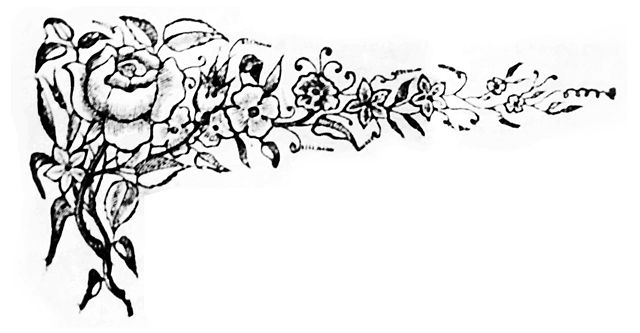
\includegraphics[width=\textwidth,height=7cm]{Kulasthree_Chapter_three_pic02.jpg}
\end{center}
%\caption*{പുലയർ - കെ പി പത്മനാഭ മേനോൻ - വാള്യം 3, (1929), 1984}
\end{figure}

\section{എന്താണീ 'മാമൂൽ?'}
\label{ch3sec2}
\paragraph{}
പണ്ടു നിലവിലുണ്ടായിരുന്ന ജാതിവ്യവസ്ഥയിൽ പാലിച്ചിരുന്ന ആചാരങ്ങൾക്കും നിയമങ്ങൾക്കും മൊത്തത്തിൽ പറയുന്ന പേരാണ് 'മാമൂൽ'. പണ്ടൊക്കെ വളരെ കണിശമായി പാലിച്ചിരുന്ന ദുരാചാരങ്ങളായ തൊട്ടുകൂടായ്മ, തീണ്ടൽ, മാസക്കുളിസമയത്തെ അശുദ്ധി കൽപിക്കലും പുറത്തു മാറിയിരിക്കലുമൊക്കെ 'മാമൂലി'ന്റെ ഭാഗമായിരുന്നു. കരമനയാറു കടന്നാൽ മേൽജാതിസ്ത്രീകളുടെ ജാതി പോകുമെന്ന വിശ്വാസവും 'മാമൂലാ'യിരുന്നു, ഇന്ന് അങ്ങനെയൊരു വിശ്വാസം നിലവിലില്ലെങ്കിലും. ഏകദേശം പത്തെഴുപതു വർഷം മുമ്പുവരെ വടക്കേ മലബാറിൽ കോരപ്പുഴ കടന്നാൽ സ്ത്രീകളുടെ ജാതി പോകുമെന്ന വിശ്വാസം നിലനിന്നിരുന്നു. ഇത്തരം ദുരാചാരങ്ങളെ പാലിച്ചു നിലനിർത്തേണ്ടത് ഇവിടത്തെ രാജകുടുംബങ്ങളുടെ കടമയായി കണക്കാക്കപ്പെട്ടിരുന്നു (രാജഭരണം വളരെ നന്നായിരുന്നുവെന്നൊക്കെ തട്ടിവിടുന്നവർ മറക്കുന്ന കാര്യം).

\begin{figure}[h]
\begin{center}
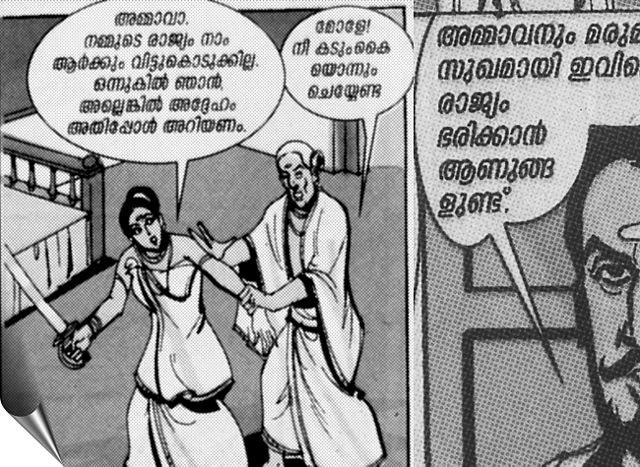
\includegraphics[width=\textwidth,height=7cm]{Kulasthree_Chapter_three_pic03.jpg}
\end{center}
%\caption*{പുലയർ - കെ പി പത്മനാഭ മേനോൻ - വാള്യം 3, (1929), 1984}
\end{figure}

\paragraph{}എന്തായാലും ഉമാകേരളത്തിലെ ദുരന്തനായികയെയല്ല നാമിവിടെ കാണുന്നത്. ഈ ഉമയമ്മറാണി ആറ്റിങ്ങൽ പ്രദേശത്ത് ഇന്നും പ്രശസ്തയത്രെ. മുതിർന്നവരോട് 'ഓർഡറി'ടുന്ന കൊച്ചുമിടുക്കികളോട് "എന്താ നീ ഉമയമ്മറാണിയാണോ?" എന്നു ചോദിക്കുന്ന രീതി ഇന്നുമുണ്ടെന്നാണ് ആ നാട്ടുകാരായ സുഹൃത്തുക്കൾ പറയുന്നത്!

\paragraph{}സ്വന്തം ഇഷ്ടാനിഷ്ടങ്ങളെ ഉപേക്ഷിച്ച് രാജ്യസേവനം നടത്തിയ ത്യാഗസ്വരൂപിണിയെയല്ല ചരിത്രരേഖകളിൽ കാണുന്നത്. മറിച്ച്, തന്റെ താൽപര്യങ്ങൾ തുറന്നു പ്രകടിപ്പിക്കാൻ മടിക്കാത്ത ഒരു വനിതയായിരുന്നു അവരെന്ന സൂചനകളുണ്ട്. (റാണിക്ക് ഇംഗ്ളീഷുകാരുമായി നല്ല ബന്ധമാണുണ്ടായിരുന്നത്. അതുകൊണ്ട് ഇത് റാണിയുടെ സൽപ്പേര് കളങ്കപ്പെടുത്താനുളള ശ്രമമായിക്കാണാൻ കഴിയില്ല) പുറവഴിനാട് കേരളവർമ്മയും റാണിയും തമ്മിൽ സംബന്ധമുണ്ടായിരുന്നെന്നും സൂചനകളുണ്ട്. അക്കാലത്ത് ഇതൊന്നും നാണക്കേടായിരുന്നില്ലെന്നും ഒന്നിലധികം ഭർത്താക്കന്മാർ സ്ത്രീകൾക്കുണ്ടാകുന്ന രീതി അന്നത്തെ പല ജാതികളിലും പതിവായിരുന്നെന്നും ചരിത്രകാരനായ കെ. ശിവശങ്കരൻ നായർ വേണാടിന്റെ പരിണാമം എന്ന കൃതിയിൽ ചൂണ്ടിക്കാണിക്കുന്നു. പക്ഷെ, ഉമാകേരളത്തിലെ ഉമയമ്മറാണി ഇങ്ങനെയുളള ആഗ്രഹങ്ങൾ പ്രകടിപ്പിക്കുന്ന സ്ത്രീയല്ല. ശരി, ഇതൊക്കെ വളരെ രസകരംതന്നെ. എങ്കിലും ഇങ്ങനെ ഒരു റാണിയെ കണ്ടെടുത്തതിൽനിന്ന് നമ്മൾ കൂടുതലായി എന്തെങ്കിലും പഠിക്കുന്നുണ്ടോ? ഉമയമ്മയെപ്പോലെ ശേഷിയും ശേമുഷിയും തികഞ്ഞവരായിരുന്നു അന്നത്തെ പെണ്ണുങ്ങളെല്ലാവരും എന്നു പറയാൻ പറ്റില്ലല്ലോ. എന്തിന്, അന്നത്തെ മേലാളസ്ത്രീകളെല്ലാവരും ഇതു പോലെയായിരുന്നെന്നുപോലും പറയാനൊക്കില്ല! സമീപകാലത്തും കാര്യങ്ങൾ മാറിയിട്ടില്ല. ഇന്ദിരാഗാന്ധി, സിരിമാവോ ബണ്ഡാരനായകെ, ബേനസീർ ഭൂട്ടോ, ഷേയ്ഖ് ഹസീന - ഇന്ത്യ, ശ്രീലങ്ക, പാകിസ്ഥാൻ, ബാംഗ്ലദേശ് എന്നീ രാജ്യങ്ങളിലെ പ്രധാനമന്ത്രിപദംവരെ എത്തിയ ഈ സ്ത്രീകളുണ്ടായതുകൊണ്ട് ഇവിടങ്ങളിലെ സ്ത്രീജനങ്ങൾക്ക് അധികാരവും അംഗീകാരവും ലഭിച്ചുവെന്ന് പറയാനാവില്ലല്ലോ. പക്ഷേ, ഉമാകേരളത്തിലെ റാണിയുടെ ചിത്രവും ചരിത്രരേഖകൾ വെളിപ്പെടുത്തുന്ന ചിത്രവും ഇത്രയും വ്യത്യസ്തമായതെന്തുകൊണ്ട് എന്നു ചോദിക്കുന്നതിലൂടെ നമുക്ക് കുറേക്കൂടി വലുതായ, ഇന്നത്തെ നമ്മുടെ ജീവിതത്തെ നേരിട്ടു സ്പർശിച്ച ഒരു ചരിത്രപ്രക്രിയയെപ്പറ്റി കൂടുതൽ അറിവുണ്ടാകുന്നു. അതായത് കേരളത്തിലെ സ്ത്രീകൾ - മേലാളസ്ത്രീകൾപോലും - രാഷ്ട്രീയാധികാരത്തിന്റെ ഉയർന്ന മേഖലകൾക്കു പുറത്തായ പ്രക്രിയയെപ്പറ്റി.

\paragraph{}ഉമയമ്മറാണി എടുത്തുപയോഗിച്ച അധികാരത്തെക്കുറിച്ചുള്ള രേഖകൾ വിരൽചൂണ്ടുന്നത് അക്കാലത്ത് ഇവിടെ നടപ്പിലുണ്ടായിരുന്ന രാഷ്ട്രീയാധികാരത്തിന്റെ ഒരു പ്രത്യേകതയിലേക്കാണ്. ഇന്ത്യയിലെ മറ്റുപ്രദേശങ്ങളിലധികവും സ്ത്രീകൾക്ക് കിരീടാവകാശം ഇല്ലായിരുന്നു. രാജാവ് അന്തരിച്ചാൽ കിരീടാവകാശിയായ കുമാരന് പ്രായപൂർത്തിയായിട്ടില്ലാത്ത സാഹചര്യമാണുള്ളതെങ്കിൽമാത്രം റാണി താൽക്കാലികചുമതലയേറ്റിരുന്നു. കുമാരൻ മുതിർന്നാലുടൻ ആ സ്ഥാനം അവസാനിക്കുകയും ചെയ്യും. ഇംഗ്ലീഷുകാർ ഈ സമ്പ്രദായത്തെ റീജൻസി (regency) എന്നു വിളിച്ചു. പക്ഷേ, കേരളത്തിൽ പലയിടത്തും ഇക്കാര്യത്തിൽ ചില വ്യത്യാസങ്ങൾ കണ്ടിരുന്നു.

\paragraph{}ബ്രിട്ടിഷുകാർ പത്തൊമ്പതാംനൂറ്റാണ്ടോടുകൂടി ഇവിടത്തെ നാട്ടുരാജ്യങ്ങളെ കീഴടക്കുന്നതിനു മുമ്പുള്ള കാര്യമാണ് പറയുന്നത് - ഉമയമ്മറാണിയുടെ കാലത്ത് ബ്രിട്ടിഷുകാർ ഇതിന് ശ്രമിച്ചു തുടങ്ങിയിട്ടേയുണ്ടായിരുന്നുള്ളു. നേരത്തെ പറഞ്ഞതുപോലെ പതിനേഴാംനൂറ്റാണ്ടിന്റെ അവസാനകാലത്ത് ഇവിടെ നിരവധി ചെറുസ്വരൂപങ്ങളാണുണ്ടായിരുന്നത്. ഇവയിൽ മിക്കവയിലും അധികാരം ഏറ്റവുംമൂത്ത പുരുഷനായിരുന്നു. എന്നാൽ പല സ്വരൂപങ്ങളിലും പുരുഷസന്തതി ഇല്ലാതെവന്ന അവസരങ്ങളിൽ മൂത്ത സ്ത്രീക്ക് ലഭിച്ചിരുന്നത് പൂർണാധികാരമായിരുന്നു - അതായത് മൂപ്പെത്താത്ത പുരുഷസന്തതിയുടെ പ്രതിനിധിയായിട്ടല്ല മൂത്ത സ്ത്രീ ഭരണംനടത്തിയിരുന്നത്. സ്വന്തംനിലയിൽത്തന്നെയായിരുന്നു. 'തമ്പുരാൻ' എന്ന പദത്തെ ഇന്നു നാം പുരുഷന്മാരോടാണ് ബന്ധപ്പെടുത്താറുള്ളത്. എന്നാൽ പണ്ട് രാജകുടുംബങ്ങളിലെ സ്ത്രീകൾക്കും പുരുഷന്മാർക്കും ഈ നാമം ബാധകമായിരുന്നു - പലപ്പോഴും മൂത്ത തമ്പുരാട്ടിയെന്നല്ല, മൂത്ത തമ്പുരാൻ എന്നാണ് ആറ്റിങ്ങൽ റാണിയെ വിശേഷിപ്പിച്ചിട്ടുളളത്. തൃപ്പാപ്പൂർ, ദേശിങ്ങനാട് എന്നീ സ്വരൂപങ്ങളുടെ മൂപ്പവകാശം ആറ്റിങ്ങൽ തമ്പുരാട്ടിമാരുടെ പുരുഷസന്തതികൾക്കായിരുന്നു. (ഇതിനെക്കുറിച്ചാണ് മുമ്പു പറഞ്ഞ യൂറോപ്യൻ സൈനികന്റെ ഉദ്ധരണി). ഇങ്ങനെ ആറ്റിങ്ങൽ തമ്പുരാട്ടിമാർക്ക് മാതൃസ്ഥാനമുണ്ടായിരുന്ന സ്വരൂപങ്ങളിൽ മൂപ്പു വാഴാൻ പുരുഷസന്താനമില്ലാതെയായാൽ, തമ്പുരാട്ടിമാർതന്നെ മൂപ്പേറിയിരുന്നതായി തെളിവുണ്ട്. ഉദാഹരണത്തിന് പതിനേഴാംനൂറ്റാണ്ടിൽ (1650കളിൽ) തൃപ്പാപ്പൂർ സ്വരൂപത്തിന്റെ മൂപ്പ് ആറ്റിങ്ങൽ മൂത്ത തമ്പുരാട്ടിയായിരുന്ന ആയില്യം തിരുനാളാണ് ഏറിയിരുന്നത്. അപ്പോൾ അവർക്കു തൊട്ടുതാഴെയുണ്ടായിരുന്ന രണ്ടാംമുറ ഇളയതമ്പുരാട്ടിയായിരുന്ന മകയിരംതിരുനാൾ ദേശിങ്ങനാട് സ്വരൂപത്തിന്റെ മൂപ്പേറിയിരുന്നു. (മുൻചൊന്ന സൈനികന്റെ ഉദ്ധരണിയിലെ മൂത്തതമ്പുരാട്ടി ഇവരായിരുന്നു). ആറ്റിങ്ങൽ റാണിമാർക്ക് പുരുഷസന്തതി ഇല്ലാതെവന്ന അവസരങ്ങളായിരുന്നു ഇവയെന്ന് കെ. ശിവശങ്കരൻ നായർ പറയുന്നു. ഇതുകൂടാതെ രണ്ടു സ്വരൂപങ്ങളിൽ - തെക്ക് ആറ്റിങ്ങലും വടക്ക് അറയ്ക്കലും - പെണ്ണുങ്ങൾ നേരിട്ട് മൂപ്പ് വാണിരുന്നു. അപ്പോൾ ഉമയമ്മയുടെ ഭരണാധികാരമോഹം നാട്ടുനടപ്പിന് അത്രയ്ക്കൊന്നും വിരുദ്ധമായിരുന്നില്ലെന്നർത്ഥം!


\paragraph{}ഇന്നത്തെ കണ്ണൂർജില്ലയിലുണ്ടായിരുന്ന അറയ്ക്കൽസ്വരൂപം ഇസ്ലാംമത വിശ്വാസികളായിരുന്നുവെങ്കിലും മക്കത്തായ കുടുംബമായിരുന്നില്ല. ഇവിടെ കാരണവസ്ഥാനം മൂത്ത സ്ത്രീ വഹിച്ചിരുന്നു. ബ്രിട്ടിഷുകാരുടെ രേഖകളിൽ പലപ്പോഴും ഇവിടത്തെ യഥാർത്ഥ ഭരണാധികാരി മൂത്ത പുരുഷന്മരായിരുന്നുവെന്ന് പറയുന്നുമുണ്ട്. പക്ഷേ, എല്ലാ രാജകീയവിളംബരങ്ങളും ഉടമ്പടികളും ഭരണാധികാരിയായ അറയ്ക്കൽബീവിയുടെ പ്രത്യക്ഷസമ്മതത്തോടുകൂടി മാത്രമേ നടപ്പിൽവരൂ എന്ന് ഈ രേഖകൾതന്നെ പറയുന്നുണ്ട്. എന്തായാലും പതിനെട്ടാംനൂറ്റാണ്ടിൽ ഇവിടെ മൂപ്പുവാണവരുടെ പട്ടികയിൽ നിരവധി ബീവിമാരുടെ പേരുകളുണ്ട്. ബ്രിട്ടിഷ്‌ രേഖകൾ പലപ്പോഴും ബീവി ഭർത്താവിന്റെ കയ്യിലാണെന്നൊക്കെ പറയുകയും മറ്റൊരുവശത്ത് ഇവർക്ക് 'ആഴിരാജ' എന്ന സ്ഥാനബിരുദമുണ്ടായിരുന്നെന്ന് പറയുകയും കുടുംബകാരണവർ ഇവരായിരുന്നെന്ന് സമ്മതിക്കുകയുംചെയ്യുന്നു. 1790കളിൽ മൈസൂർ സുൽത്താൻ ടിപ്പുവിനെ ബ്രിട്ടിഷുകാർ തോൽപ്പിച്ചതോടെ മലബാറിലെ എല്ലാ സ്വരൂപങ്ങളും അവരുടെ അധീനതയിലായി. അറയ്ക്കൽ സ്വരൂപത്തിനും സ്വതന്ത്രനില നഷ്ടമായി. പക്ഷേ, ബീവിമാർ കാരണവസ്ഥാനത്തെത്തുന്ന പതിവ് നഷ്ടമായില്ല.

\captionof{mybox}{ഇന്ത്യ, ബ്രിട്ടിഷ് ഭരണാധികാരികളുടെ കണ്ണിൽ}\label{ch3box2} % place the caption
\begin{tcolorbox}[%
 breakable, % make the box breakable
  arc=0mm, 
  left=1pt, right = 1pt, 
  boxrule=0mm,
  colback = {blue!10}, % since shadow-gray was not defined
] 
നിരവധി സംസ്കാരങ്ങളും ഭാഷകളും ഭരണരീതികളും കുടുംബരൂപങ്ങളും മറ്റും കൂടിച്ചേർന്ന് നിലനിന്നിരുന്ന ഇന്ത്യയിലേക്കാണ് ബ്രിട്ടിഷുകാർ ഭരണാധികാരികളായി വന്നത്. ഇവിടത്തെ അമ്പരപ്പിക്കുന്ന വൈവിദ്ധ്യം ഭരണതാത്പര്യങ്ങൾക്ക് വിലങ്ങുതടിയായി അനുഭവപ്പെട്ടു. ഇന്ത്യൻ സംസ്കാരത്തിനും ജനതയ്ക്കും പുറമെകാണുന്ന വൈവിദ്ധ്യത്തിനു കീഴിലായി ഏകസ്വഭാവമാണുള്ളതെന്നും ആ അന്തഃസത്ത കണ്ടെത്തി ഭരണത്തെ അതിനനുസൃതമായി ചിട്ടപ്പെടുത്തണമെന്നും ബ്രിട്ടിഷ് ഭരണാധികാരികളിൽ ഒരു പ്രബലവിഭാഗം വാദിച്ചു. അവർക്ക് പിൻബലമായത് 'പൗരസ്ത്യവാദം' (orientalism) എന്ന ജ്ഞാനശാഖയായിരുന്നു. ഇന്ത്യയടക്കമുള്ള കിഴക്കൻ സംസ്കാരങ്ങളെക്കുറിച്ച് നിരവധി നൂറ്റാണ്ടുകളായി പാശ്ചാത്യഗവേഷകർ നടത്തിവന്ന പഠനഗവേഷണപ്രവർത്തനങ്ങളിലൂടെ ഉരുത്തിരിഞ്ഞുവന്ന 'പൗരസ്ത്യവാദം' കിഴക്കൻ സമൂഹങ്ങളുടെ വൈവിദ്ധ്യത്തെ മായ്ച്ചുകളയുകയും ഒപ്പം വ്യത്യസ്തതയുടെ ചില വാർപ്പുമാതൃകകൾ (stereotypes)ക്കുള്ളിൽ അവയെ തളയ്ക്കുകയും ചെയ്തു. ഇവ ബ്രിട്ടിഷ് ഭരണയന്ത്രത്തിലൂടെ സ്ഥാപനവൽക്കരിക്കപ്പെട്ടു (ഇന്ത്യയിൽ സ്ത്രീകൾക്ക് പൂർണ്ണ രാജാധികാരത്തിന് അവകാശമില്ലെന്ന ധാരണ ഇത്തരമൊരു വാർപ്പുമാതൃകയിൽനിന്ന് ഉണ്ടായതാണ്). സ്വാതന്ത്ര്യാന്തരകാലത്തുപോലും നാം ഇവയുടെ പിടിയിൽനിന്ന് പൂർണ്ണമായി രക്ഷപെട്ടിട്ടില്ല എന്നതാണ് വാസ്തവം. അധിനിവേശവും ദേശീയതയും തമ്മിലുള്ള ഇത്തരം പങ്കുവയ്ക്കലുകളെ ഗൗരവത്തോടുകൂടി പഠിക്കേണ്ടതാണെന്ന് അധിനിവേശാനന്തര ചരിത്രരചനയുടെ വക്താക്കൾ നിരീക്ഷിക്കുന്നു.
\end{tcolorbox}

\begin{figure}
\begin{center}
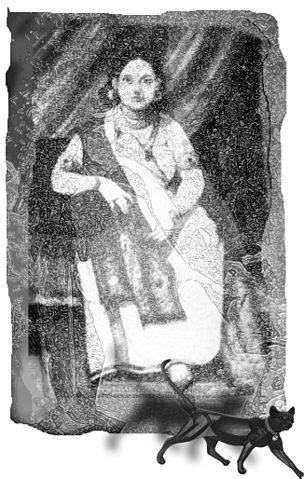
\includegraphics[width=\textwidth,height=10cm]{Kulasthree_Chapter_three_pic04.jpg}
\end{center}
%\caption*{പുലയർ - കെ പി പത്മനാഭ മേനോൻ - വാള്യം 3, (1929), 1984}
\end{figure}

\paragraph{}തെക്ക് ഇതായിരുന്നില്ല അനുഭവം. ഇവിടെ ബ്രിട്ടിഷുകാർ അധികാരത്തിലെത്തുംമുമ്പുതന്നെ ഭരണാധികാരിണികളുടെ സ്വതന്ത്രനിലയ്ക്ക് കോട്ടമുണ്ടായി. പതിനെട്ടാംനൂറ്റാണ്ടിൽ, ഇന്നത്തെ കേരളത്തിന്റെ തെക്കൻപ്രദേശങ്ങളിലെ സ്വരൂപങ്ങളെ തിരുവിതാംകൂറിലെ മാർത്താണ്ഡവർമ്മ ആക്രമിച്ച് കീഴടക്കി ഒരൊറ്റ രാജ്യമാക്കി. ആറ്റിങ്ങൽ സ്വരൂപത്തിന്റെയും സ്വതന്ത്രനില ഇല്ലാതായി. മുമ്പ് ആറ്റിങ്ങൽറാണിമാർക്ക് ഏകദേശം 15,000 ഏക്കർ വിസ്തീർണംവരുന്ന പ്രദേശങ്ങൾക്കുമേൽ അധികാരമുണ്ടായിരുന്നു. വിദേശീയരുമായി സ്വതന്ത്ര ഉടമ്പടികളും മറ്റുമുണ്ടാക്കാനുള്ള അധികാരമുണ്ടായിരുന്നു. വാണിജ്യകാര്യങ്ങളിലും ആറ്റിങ്ങൽ റാണി സ്വതന്ത്രയായിരുന്നെന്നും ചരിത്രരേഖകൾ വെളിപ്പെടുത്തുന്നു. ഈ മാർത്താണ്ഡവർമ്മ ഒരു ആറ്റിങ്ങൽ തമ്പുരാട്ടിയുടെ മകനായിരുന്നു. അദ്ദേഹം തമ്പുരാട്ടിമാരുമായി 1747ൽ നടത്തിയ ഉടമ്പടിപ്രകാരം ആറ്റിങ്ങൽസ്വരൂപം പൂർണ്ണമായും തിരുവിതാംകൂറിന്റെ ഭാഗമായി. ഭാവിയിൽ തിരുവിതാംകൂർ വാഴുന്ന രാജാക്കന്മാരെല്ലാവരും ആറ്റിങ്ങൽ റാണിമാരുടെ സന്തതികളായിരിക്കുമെന്ന ഉറപ്പും മാർത്താണ്ഡവർമ്മ നൽകി. ആറ്റിങ്ങൽ തമ്പുരാട്ടിമാർ ഭരണാധികാരികളല്ലാതെയായി. തിരുവിതാംകൂർ രാജാവിന്റെ മാതാക്കൾ എന്ന സ്ഥാനത്തേക്ക് അവരുടെ നില ചുരുങ്ങി (തന്റെ അമ്മമാരായ ആറ്റിങ്ങൽ റാണിമാരെ കൂടുതൽ നന്നായി സേവിക്കാനാണ് ഇതു ചെയ്യേണ്ടിവന്നതെന്ന് മാർത്താണ്ഡവർമ്മ അവകാശപ്പെട്ടത്രെ!). ചുരുക്കിപ്പറഞ്ഞാൽ, റാണിമാരായിരുന്നവർ വെറും അമ്മത്തമ്പുരാട്ടിമാരായി.

\paragraph{}ബ്രിട്ടിഷുകാർ അധികാരത്തിലെത്തിയത് മാർത്താണ്ഡവർമ്മയ്ക്കും അദ്ദേഹത്തിന്റെ പിന്മുറക്കാരനായിരുന്ന രാമവർമ്മ ധർമ്മരാജാവിനും ശേഷമായിരുന്നു. ബ്രിട്ടിഷുകാരുടെ ചരിത്രത്തിൽ സ്വന്തം നിലയിൽ രാജ്യംവാണ റാണിമാരുണ്ടായിരുന്നുവെന്നതൊക്കെ നേരുതന്നെ. (എലിസബത്ത് മഹാറാണി, വിക്ടോറിയ മഹാറാണി, രണ്ടാം എലിസബത്ത് മഹാറാണി) പക്ഷേ, ഇവിടെ എത്തിയപ്പോൾ ഇവിടത്തെ രാജാക്കന്മാരുടെ സമ്പ്രദായങ്ങൾ കഴിവതും നിലനിർത്തണമെന്ന അഭിപ്രായമായിരുന്നു പല ബ്രിട്ടിഷ് ഭരണാധികാരികൾക്കും. ഇന്ത്യൻ പ്രവിശ്യകളിലെ ഭരണാധികാരരീതികളെ കാക്കണമെന്ന് അവർക്കു തോന്നിയത് നമ്മോടുള്ള സ്നേഹംകൊണ്ടൊന്നുമല്ല; മറിച്ച് അവരുടെ ഭരണസൗകര്യത്തിനുവേണ്ടിയായിരുന്നു. എന്നാൽ ഇന്ത്യയിൽത്തന്നെ പല പ്രദേശങ്ങളിലും പല സമ്പ്രദായങ്ങൾ നിലവിലുണ്ടായിരുന്നതൊന്നും അവർ പരിഗണിച്ചില്ല.
\paragraph{}പക്ഷേ, ഒറ്റനോട്ടത്തിൽ അങ്ങനെ തോന്നുമായിരുന്നില്ല. രാമവർമ്മ ധർമ്മരാജാവിന്റെ മരണശേഷം വളരെ താമസംകൂടാതെ തിരുവിതാംകൂർ ബ്രിട്ടിഷുകാരുടെ പിടിയിലമർന്നു. വേലുത്തമ്പി മുതലായവരെ അമർച്ച ചെയ്തശേഷം തങ്ങളുടെ താത്പര്യങ്ങൾക്ക് വഴങ്ങിനിൽക്കുന്ന ഒരു രാജാവിനെ വാഴിക്കുകയെന്നതായിരുന്നു ബ്രിട്ടീഷ് അധികാരികളുടെ ലക്ഷ്യം. അന്ന് കിരീടാവകാശം ഉന്നയിച്ച തമ്പുരാനെ ബ്രിട്ടീഷുകാർ സംശയത്തോടെയാണ് കണ്ടത്. അപ്പോൾ അദ്ദേഹത്തെ വാഴിക്കുന്നതിന് പകരം ആറ്റിങ്ങൽ മൂത്തതമ്പുരാട്ടിയായിരുന്ന ഗൗരിലക്ഷ്മിഭായിയെയാണ് അവർ വാഴിച്ചത്. 1791ൽ ജനിച്ച റാണി ഗൗരീലക്ഷ്മീഭായി ആറ്റിങ്ങൽ മൂത്തതമ്പുരാട്ടിയായിരുന്ന അത്തംതിരുനാളിന്റെ മകളായിരുന്നു. ഇരുപതുവയസ്സിൽ താഴെ പ്രായമുണ്ടായിരുന്ന ഇവർ, ബ്രിട്ടിഷുകാരുടെ സമ്മർദ്ദത്തിനു വഴങ്ങിവന്നതാണെന്ന് തോന്നുന്നില്ല. മറിച്ച്, ഈ പിന്തുടർച്ചാത്തർക്കത്തിൽ അവർ സജീവപങ്കാളിയായിരുന്നെന്ന് തോന്നുന്നു. മാമൂലുകളെ അവഗണിച്ചുകൊണ്ട് ബ്രിട്ടിഷ് സർക്കാറിന്റെ പ്രതിനിധിയായിരുന്ന കേണൽ മൺറോയെ അവർ തന്റെ വസതിയിലേക്ക് വിളിച്ചുവരുത്തി അവകാശവാദം ഉന്നയിക്കുകയായിരുന്നത്രെ. തന്റെ കുടുംബത്തിന് ലഭിക്കേണ്ടതായ അധികാരം നഷ്ടമാക്കാൻ താൻ ഉദ്ദേശിക്കുന്നില്ലെന്ന് അവർ മൺറോയെ അറിയിച്ചുവെന്ന് അദ്ദേഹം ബ്രിട്ടിഷ് സർക്കാറിനെഴുതി. പക്ഷേ, റാണിയെ റീജന്റ് മാത്രമായാണ് ബ്രിട്ടിഷുകാർ കണ്ടത്. റാണിയും അതിന് വഴങ്ങിക്കൊടുത്തു. താനൊരു അബലയായ സ്ത്രീയായതു കൊണ്ട് ഭരണകാര്യങ്ങളിൽ സഹോദരനെപ്പോലെ താൻ ബഹുമാനിക്കുന്ന ബ്രിട്ടിഷ് റെസിഡന്റ് (ബ്രിട്ടിഷ് സർക്കാരിന്റെ പ്രതിനിധി) മൺറോയുടെ ഉപദേശം സ്വീകരിക്കാനാണ് താൻ ഉദ്ദേശിക്കുന്നതെന്ന് അവർ പരസ്യമായി പ്രഖ്യാപിച്ചു. ഗൗരിലക്ഷ്മീഭായി വെറും റീജന്റ് ആയിരുന്നതുകൊണ്ടാണ് അവരുടെ മകനായ സ്വാതിതിരുനാളിന് 'ഗർഭശ്രീമാൻ', അഥവാ അമ്മയുടെ ഗർഭത്തിൽ കിടന്നപ്പോഴേ രാജാവായ ആൾ എന്ന പേരുവീണത്. മകൻ പ്രായമാകുംമുമ്പ് ഗൗരിലക്ഷ്മീഭായി മരിച്ചതിനു ശേഷം അവരുടെ അനുജത്തിയായിരുന്ന ഗൗരിപാർവ്വതീഭായി ഭരണമേറ്റു. 1802ൽ ജനിച്ച ഗൗരി പാർവ്വതിഭായി അത്തംതിരുനാളിനുശേഷം ആറ്റിങ്ങൽ മൂത്തതമ്പുരാട്ടിയായി സ്ഥാനമേറ്റ ഭരണിതിരുനാളിന്റെ മകളായിരുന്നു. സ്വാതിതിരുനാളിന് പ്രായപൂർത്തിയായതോടുകൂടി അദ്ദേഹം രാജാവായി. റാണിമാരുടെ അധികാരത്തെ കുറേക്കൂടി ഇല്ലാതാക്കാനാണ് ബ്രിട്ടിഷ്ഭരണം സഹായിച്ചതെന്നു സാരം. റാണിമാർക്ക് സ്വന്തമായ അധികാരമുണ്ടാവില്ലെന്നും റീജന്റ് സ്ഥാനംമാത്രമേ ലഭിക്കൂ എന്നും ബ്രിട്ടിഷ്ഭരണത്തോടെ തീർച്ചയായി.

\paragraph{}മൂപ്പുവാണ തമ്പുരാട്ടിയുടെ സ്വന്തമായ നില ഇല്ലാതായെങ്കിലും പഴയ പ്രതാപത്തിന്റെ ചില അംശങ്ങളും ചിഹ്നങ്ങളും അപ്പോഴും ബാക്കിനിന്നിരുന്നു. 1819ൽ ഗൗരിപാർവ്വതീഭായിയുടെ രാജസഭ സന്ദർശിച്ച ബ്രിട്ടിഷ് ഉദ്യോഗസ്ഥൻ കേണൽ വാൾഷിന്റെ നിരീക്ഷണം ഇതാ:
\begin{quotation}
\noindent ആ സഭയിൽ കണ്ട രംഗം വളരെ സന്തോഷപ്രദമായിരുന്നു. നാട്ടിലെ പ്രമാണിമാർ എല്ലാവരും ബ്രിട്ടിഷ് സർക്കാറിന്റെ പ്രതിനിധികളെ ഉപചാരപൂർവ്വം സ്വീകരിക്കാൻ എത്തിയിരുന്നു. പക്ഷേ, റാണിയും യൂറോപ്യന്മാരുമൊഴികെ ഒരൊറ്റ കുഞ്ഞുപോലും ഇരുന്നില്ല. അടുത്തിടെ വിവാഹിതയായ ചെറിയതമ്പുരാട്ടിയാകട്ടെ, അവരുടെ ഭർത്താവാകട്ടെ, റാണിയുടെ അച്ഛനാകട്ടെ, ഭർത്താവാകട്ടെ, മുൻ റാണിയുടെ വിധുരനാകട്ടെ, ദിവാൻ, പ്രധാനമന്ത്രി ഇവരാകട്ടെ - ആരും ഇരുന്നില്ല.
\flushright{(പി.ശങ്കുണ്ണി മേനോൻ, ഹിസ്റ്ററി ഒഫ് ട്രാവൻകൂർ, തിരുവനന്തപുരം, 1983 -ആദ്യം പ്രസിദ്ധീകരിച്ചത് 1878, പുറം 289)}
\end{quotation}

\paragraph{}പക്ഷേ, ഇതു പൊയ്പ്പോയ പ്രതാപത്തിന്റെ ശേഷിപ്പുമാത്രമായിരുന്നു. ഇരുപതാംനൂറ്റാണ്ടിൽ റാണിമാരുടെ അധികാരമില്ലായ്മ കൂടുതൽ വെളിച്ചത്തായി. 1924ൽ തിരുവിതാംകൂർ രാജാവായിരുന്ന ശ്രീമൂലംതിരുനാൾ അന്തരിച്ചപ്പോൾ അദ്ദേഹത്തിന്റെ പിന്മുറക്കാരനായിരുന്ന ചിത്തിരതിരുനാൾ കേവലം ബാലനായിരുന്നു. അന്നത്തെ ആറ്റിങ്ങൽ മൂത്തതമ്പുരാട്ടിയായിരുന്ന സേതുലക്ഷ്മി റീജന്റ് മഹാറാണിയായി. (റീജന്റ് റാണിയായത് ചിത്തിരതിരുന്നാളിന്റെ മാതാവല്ലെന്നത് ശ്രദ്ധേയമാണ്)
ആറ്റിങ്ങൽ മൂത്തതമ്പുരാട്ടി റീജന്റ് അല്ലെന്ന് പല പത്രങ്ങളും ചൂണ്ടിക്കാട്ടി. അന്നത്തെ മലയാളമനോരമ ഇങ്ങനെ എഴുതി:
\begin{quotation}
\noindent ശ്രീചിത്തിരതിരുന്നാൾ തിരുമനസ്സിലേക്ക് പ്രായപൂർത്തിയാകുംവരെ ആറ്റിങ്ങൽ മൂത്തതമ്പുരാൻ തിരുമനസ്സുകൊണ്ട് ഭരണാധികാരിയായിരിക്കുന്നതാണ്. അവിടത്തെ അധികാരം അവിഭാജ്യമായിക്കാണണമെന്നും ആകുന്നു ഈ രാജ്യത്തെ ഭൂരിപക്ഷം ആളുകളുടെയും അഭിപ്രായം. ഈ അഭിപ്രായം കീഴ്‌നടപ്പിനും മരുമക്കത്തായ നിയമത്തിനും അനുസരണമായിത്തന്നെ ഇരിക്കുന്നു. മരുമക്കത്തായ നിയമപ്രകാരം പ്രായപൂർത്തിയായ പുരുഷന്മാരുണ്ടെങ്കിൽ അവർ കുടുംബഭരണം നടത്തുന്നതും അവരുടെ അഭാവത്തിൽ വയസ്സ് മൂപ്പുളള സ്ത്രീ കാരണവത്തിയായിരിക്കുന്നതുമാണ്. കാരണവത്തി കുടുംബഭരണം നടത്തുന്നത് ഭാവിയിൽ കാരണവൻ ആകുന്ന പുരുഷന്റെ പ്രതിനിധിയെന്ന നിലയിലല്ല. കുടുംബത്തിലെ മൂത്തയാൾ എന്ന നിലയിലാണ്. ഇങ്ങനെ വയസ്സുമൂപ്പുളള സ്ത്രീ കാരണവത്തിയായിരിക്കുന്നിടേത്താളംകാലം സ്വന്തംനിലയിൽത്തന്നെ ഭരണാധികാരിയായിരിക്കുന്നതുമാണ്. ഹിന്ദുനിയമപ്രകാരമുളള അവകാശക്രമം ഇതിൽനിന്ന് വ്യത്യസ്തമായിരിക്കുന്നു. [അതിൽ] സ്ത്രീകൾ ഭരണം നടത്തുന്നുവെങ്കിൽ, പുരുഷന്മാരുടെ പ്രതിനിധികളെന്ന നിലയിലാണ്. വാസ്തവത്തിൽ മരുമക്കത്തായമനുസരിച്ച് സ്ത്രീകൾ കുറച്ചുകാലത്തേക്കുമാത്രം കാരണവത്തികളായിരുന്നാലും അവർ ഭരണംനടത്തുന്നത് സ്വാധികാരമനുസരിച്ചാണെന്നതിന് സംശയമില്ല.
\flushright{(മലയാള മനോരമ, ആഗസ്റ്റ് 30, 1924)}
\end{quotation}



\paragraph{}ഈ വാദമൊന്നും വിലപ്പോയില്ലെന്ന് പ്രത്യേകം പറയേണ്ടതില്ല. ആറ്റിങ്ങൽ മൂത്തതമ്പുരാട്ടി വെറും റീജന്റായി സ്ഥാനമേറ്റു. ഇക്കാലമായപ്പോഴേക്കും തിരുവിതാംകൂറിൽ ജനകീയഭരണത്തിന്റെ ആരംഭം കണ്ടുതുടങ്ങിയിരുന്നു. വലിയ അധികാരമൊന്നുമില്ലായിരുന്നെങ്കിലും തിരുവിതാംകൂറിൽ ഒരു ജനപ്രതിനിധിസഭ അപ്പോഴേക്കും രൂപം കൊണ്ടു കഴിഞ്ഞിരുന്നു. 1920കളിൽ തിരുവിതാംകൂറിലെ സ്ത്രീകൾക്ക് പരിമിതമായ വോട്ടവകാശം ലഭിച്ചിരുന്നു. ബ്രിട്ടിഷ് ഇന്ത്യയിൽ സ്ത്രീകൾ ഈ അവകാശങ്ങൾക്കുവേണ്ടി മുറവിളികൂട്ടിയിരുന്ന കാലത്താണിത്.



\captionof{mybox}{റാണിമാരുടെ പോര്}\label{ch3box3} % place the caption
\begin{tcolorbox}[%
 breakable, % make the box breakable
  arc=0mm, 
  left=1pt, right = 1pt, 
  boxrule=0mm,
  colback = {blue!10}, % since shadow-gray was not defined
] 

\begin{center}
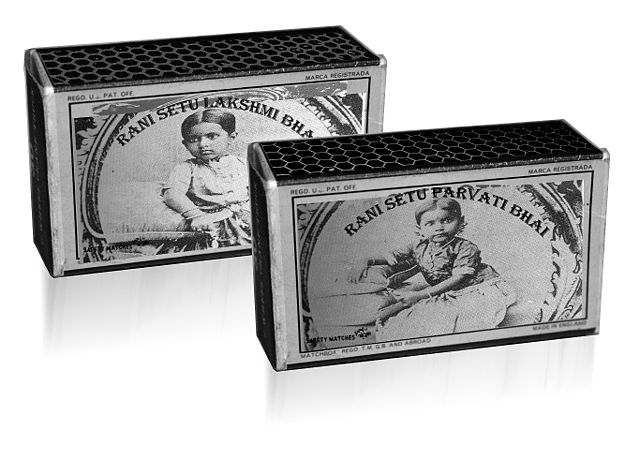
\includegraphics[width=0.5\textwidth,height=5cm]{Kulasthree_Chapter_three_pic05.jpg}
\end{center}

1930കളിൽ തിരുവിതാംകൂറിലെ റീജന്റ് മഹാറാണി സേതുലക്ഷ്മീഭായിയും കിരീടാവകാശിയായ ശ്രീചിത്തിരതിരുനാളിന്റെ മാതാവ് ഇളയറാണി സേതുപാർവ്വതീഭായിയും തമ്മിലുള്ള കിടമത്സരത്തെക്കുറിച്ചുള്ള കഥകൾ നാട്ടിലെങ്ങും പാട്ടായിരുന്നു. ബ്രിട്ടീഷ് ഇന്ത്യയിലെ സമ്പ്രദായപ്രകാരം കിരീടാവകാശിയുടെ അമ്മ മഹാറാണിയായി താത്കാലികചുമതലയേൽക്കുന്ന രീതി ഇവിടെ സ്വീകരിക്കാത്തതിൽ പാർവ്വതീഭായിക്ക് പ്രതിഷേധമുണ്ടായിരുന്നത്രെ. തിരുവിതാംകൂറിൽ നടപ്പുണ്ടായിരുന്ന രീതി പ്രകാരമാണ് മൂത്തതമ്പുരാട്ടി റീജന്റായത്. ഈ വിരോധം പിന്നീട് രൂക്ഷമായെന്നാണ് നാട്ടുവർത്തമാനം - അന്നത്തെ സംഭവങ്ങൾക്ക് ദൃക്‌സാക്ഷിയായിരുന്ന ലൂയിസ് ഔവർക്കർക്ക് എന്ന ഡച്ച് വനിത 1930കളിലെ തിരുവിതാംകൂർ രാഷ്ട്രീയത്തെക്കുറിച്ച് എഴുതിയ പുസ്തകത്തിൽ ഈ തർക്കത്തെക്കുറിച്ച് പരാമർശിക്കുന്നുണ്ട്.

\end{tcolorbox}

\paragraph{}
എന്നാൽ തിരുവിതാംകൂറിൽ സ്ത്രീകളെ പൂർണ്ണനിലയിൽ ഭരണാധികാരികളായി കാണുന്നതിനോടുളള എതിർപ്പ് കുറഞ്ഞുവെന്നു പറയാനാവില്ല. 'സ്ത്രീസ്വഭാവ'ത്തെക്കുറിച്ച് പുതിയ ആശയങ്ങൾ പ്രചരിച്ചുതുടങ്ങിയ കാലമാണിത്. 'അടുക്കളയിൽനിന്ന് അരങ്ങത്തേക്കി'റങ്ങാൻ സ്ത്രീകളെ സഹായിച്ച കേരളത്തിലെ സാമുദായികപ്രസ്ഥാനങ്ങളെപ്പറ്റി നാം വളരെ കേൾക്കാറുണ്ട്. പക്ഷേ, സമുദായപരിഷ്കർത്താക്കളിൽ നല്ലൊരു വിഭാഗം സ്ത്രീകളെ 'കുടുംബത്തിന്റെ വിളക്കുകൾ' മാത്രമായി കാണാൻ ആഗ്രഹിച്ചിരുന്നവരായിരുന്നു. അധികാരത്തോടടുക്കുന്ന സ്ത്രീകളെ അവർ സംശയത്തോടെ കണ്ടു. 'അമ്മത്തമ്പുരാട്ടി'കളും 'ത്യാഗമൂർത്തി'കളുമായ സ്ത്രീകളെ മാത്രമേ അധികാരത്തിന്റെ ഉന്നതങ്ങളിൽ അവർ കണ്ടിരുന്നുള്ളു. പുരുഷന്മാരെപ്പോലെ അധികാരം കയ്യാളുന്ന സ്ത്രീ ദുഷ്ടയും 'പൗരുഷക്കാരി'യുമായിരിക്കും എന്ന മുൻവിധി, നാമിന്ന് ആരാധിക്കുന്ന പല സമുദായപരിഷ്കർത്താക്കളായ മഹാന്മാരും വച്ചുപുലർത്തിയിരുന്നു. 1930കളിൽ നമ്പൂതിരിസമുദായ പരിഷ്കരണപ്രസ്ഥാനത്തിലും അതിനുശേഷവും സമുദായപരിഷ്കർത്താക്കളായി ഉയർന്നുവന്ന പലരും സ്ത്രീകളുടെ സാമൂഹ്യപദവിയെക്കുറിച്ച് വിശാലമായ നിലപാടു സ്വീകരിക്കാൻ ശ്രമിച്ചുവെങ്കിലും സ്ത്രീകളുടെ രാഷ്ട്രീയപ്രവേശത്തെക്കുറിച്ച് അവർ പുലർത്തിയ നിലപാടുകൾ അത്രയൊന്നും സഹായകമായിരുന്നില്ല. തിരുവിതാംകൂർ നിയമസഭയിലേക്ക് നാമനിർദ്ദേശം ചെയ്യപ്പെട്ട സ്ത്രീകളും അവരെപ്പോലെ രാഷ്ട്രീയത്തിൽ താത്പര്യമുണ്ടായിരുന്നവരുമായ സ്ത്രീകളും 'പുരുഷന്മാരെപ്പോലെ' ആകാൻ ആഗ്രഹിക്കുന്നവരാണെന്നുപോലും പ്രചരണമുണ്ടായി; ഉത്തമസ്ത്രീ രാജ്യഭരണത്തിനിറങ്ങില്ലെന്നും കുടുംബഭരണംകൊണ്ട് തൃപ്തയാവുമെന്നും. അധികാരം ആഗ്രഹിക്കുന്ന സ്ത്രീ 'ഒട്ടും ശരിയല്ലെ'ന്നുവന്ന ഈ പശ്ചാത്തലത്തിൽ ശരിക്കും ശക്തിസ്വരൂപിണിയായി ചരിത്രരേഖകളിൽ പ്രത്യക്ഷപ്പെടുന്ന ഉമയമ്മറാണി ഉമാകേരളത്തിൽ വൻദുരന്തംസഹിച്ച സാധ്വിയും ദേശഭക്തയുമായ മാതാവായി ചുരുങ്ങിയതിൽ അതിശയിക്കാനൊന്നുമില്ലല്ലോ.


\captionof{mybox}{വോട്ടവകാശത്തിനായി സ്ത്രീകൾ മുന്നിട്ടിറങ്ങുന്നു}\label{ch3box2} % place the caption
\begin{tcolorbox}[%
 breakable, % make the box breakable
  arc=0mm, 
  left=1pt, right = 1pt, 
  boxrule=0mm,
  colback = {blue!10}, % since shadow-gray was not defined
] 

\begin{center}
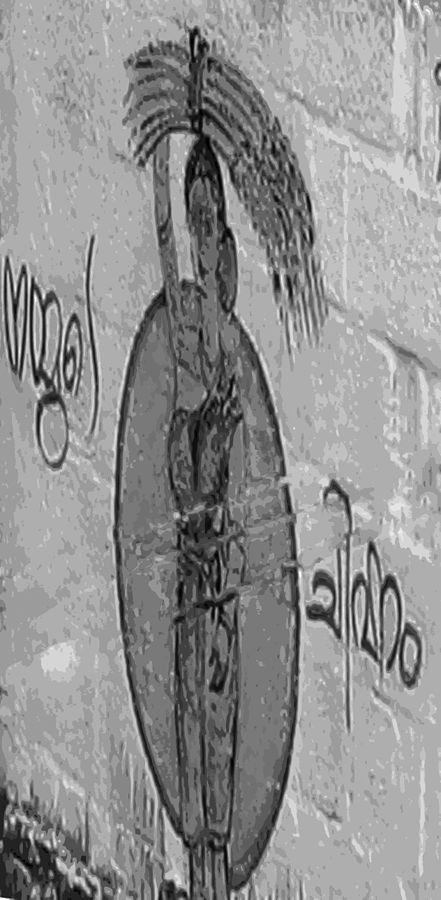
\includegraphics[width=0.5\textwidth,height=5cm]{Kulasthree_Chapter_three_pic06.jpg}
\end{center}


1917ൽ ബ്രിട്ടിഷ് ഇന്ത്യയിലെ ഭരണസംവിധാനത്തിൽ കൂടുതൽ ഇന്ത്യക്കാരെ ഉൾപ്പെടുത്തുമെന്ന് ഔദ്യോഗിക പ്രഖ്യാപനമുണ്ടായതിനെത്തുടർന്ന് ഇന്ത്യൻജനതയുടെ അഭിപ്രായമാരായാൻ അന്നത്തെ വൈസ്രായിയുൾപ്പെടെയുള്ള രണ്ടംഗസംഘം ഇന്ത്യാപര്യടനം നടത്തി. ഇത് ഒരവസരമായിക്കണ്ട അന്നത്തെ അഭ്യസ്തവിദ്യരായ ഇന്ത്യൻ സ്ത്രീകൾ - ബംഗാൾ, മദ്രാസ് തുടങ്ങിയ സ്ഥലങ്ങളിൽ ചില സ്ത്രീസംഘടനകൾ പ്രവർത്തിച്ചിരുന്നു - ഈ പ്രതിനിധിസംഘത്തെ നേരിട്ടുകണ്ട് തങ്ങളുടെ രാഷ്ട്രീയ അവകാശങ്ങളുന്നയിക്കാൻ മുതിർന്നു. ബംഗാളിലെ ഭാരതസ്ത്രീമണ്ഡലത്തെ പ്രതിനിധീകരിച്ച് സരളാദേബി ചൗധുറാണിയും മദ്രാസിൽനിന്ന് വിമൻസ് ഇന്ത്യൻ അസോസിയേഷനെ പ്രതിനിധീകരിച്ച് മാർഗരറ്റ് കസിൻസും കൂടിക്കാഴ്ചയ്ക്കായി അപേക്ഷ നൽകി. രാഷ്ട്രീയസ്വഭാവമുള്ള കാര്യങ്ങൾ ചർച്ചചെയ്യാനുദ്ദേശിക്കുന്നവരെ മാത്രമേ സംഘം കാണുകയുള്ളുവെന്ന മറുപടിയാണ് കസിൻസിനു ലഭിച്ചത്. തങ്ങളുന്നയിക്കാനിരിക്കുന്ന കാര്യം തികച്ചും രാഷ്ട്രീയസ്വഭാവമുള്ളതാണെന്ന് അവർ വാദിച്ചു. ഒടുവിൽ ദീർഘകാലകോൺഗ്രസ്പ്രവർത്തകയും അറിയപ്പെട്ട കവിയുമായ സരോജിനി നായിഡുവിന്റെ നേതൃത്വത്തിൽ അഖിലേന്ത്യാസ്വഭാവമുള്ള ഒരു സ്ത്രീസംഘം ബ്രിട്ടിഷ്സംഘത്തെ കണ്ടു. ഇന്ത്യയിലെ മുഴുവൻ സ്ത്രീകൾക്കുംവേണ്ടിയാണ് തങ്ങൾ വാദിക്കുന്നതെന്ന് ഇവർ അവകാശപ്പെട്ടു. പക്ഷേ, നിവേദനങ്ങൾ, പൊതുയോഗങ്ങൾ, പ്രമേയങ്ങൾ മുതലായവ വഴി വളരെ ശക്തമായ സമ്മർദ്ദം ചെലുത്തിയിട്ടും സ്ത്രീകളുടെ അവകാശവാദങ്ങളെ സർക്കാർ അവഗണിക്കുകയാണുണ്ടായത്.

\end{tcolorbox}

\paragraph{}

രാജ്യസേവനത്തിൽ സ്ത്രീകൾ ഉണ്ടാകണമെന്നും അവർ യാതൊരുവിധ അധികാരമോഹവുമില്ലാതെ കേവലം സേവനത്തിനുവേണ്ടിമാത്രം പ്രവർത്തിക്കണമെന്നും ഉപദേശിക്കാൻ അന്നത്തെ മഹാന്മാർ പലരും മറന്നില്ല. ചുരുക്കിപ്പറഞ്ഞാൽ സ്ത്രീകളുടെ രാഷ്ട്രീയ പ്രവർത്തനം സാമൂഹ്യസേവനംമാത്രമാണെന്നും അതിലൂടെ അവർ അധികാരത്തിലെത്താമെന്നൊന്നും മോഹിക്കേണ്ടതില്ലെന്നും വന്നു. സേവനമനഃസ്ഥിതിയാണ് സ്ത്രീകളുടെ മുഖ്യഗുണമെന്ന് നാം ഇന്നും എന്നും കേൾക്കുന്ന ആ പല്ലവി അന്നുതന്നെ സ്ത്രീകളെ രാഷ്ട്രീയത്തിന്റെ പിൻനിരയിലേക്ക് തള്ളാൻ നല്ലൊരു ആയുധമായി മാറിക്കഴിഞ്ഞിരുന്നു. സ്വാതന്ത്ര്യം കിട്ടിയതിനുശേഷം കേരളത്തിൽ നടന്ന അധികാരമത്സരങ്ങളിൽ കഴിവുറ്റ സ്ത്രീകൾ പലരും പുറത്തായി. സ്വാതന്ത്ര്യത്തിന്റെ ആദർശമെല്ലാം പതുക്കെ തണുത്തു. തിരഞ്ഞെടുപ്പിന്റെ ഗോദയിലേക്ക് കടന്നപ്പോൾ കേരളത്തിലെ കോൺഗ്രസ്സിന്റെ പിതാമഹന്മാരും സമുദായനേതാക്കന്മാരും സ്ത്രീകൾക്കു പറ്റിയ രംഗമല്ല രാഷ്ട്രീയം എന്നുവരെ പ്രഖ്യാപിച്ചു. ദേശീയതലത്തിൽ ജവഹർലാൽ നെഹ്രു കോൺഗ്രസ്സ് സ്ഥാനാർത്ഥിപ്പട്ടികയിൽ സ്ത്രീകൾക്ക് പതിനഞ്ചു ശതമാനം സീറ്റ് സംവരണം നൽകണമെന്ന് വാദിച്ചതിനു പുറകെയായിരുന്നു ഇത്. തിരു-കൊച്ചിയിൽ കോൺഗ്രസ്സ് സ്ഥാനാർത്ഥിപ്പട്ടികയിൽ സ്ത്രീകളുടെ എണ്ണം കുറഞ്ഞുപോയതിനെക്കുറിച്ച് ഇവിടത്തെ തലമൂത്ത രാഷ്ട്രീയനേതാക്കളിൽ ഒരാളായിരുന്ന കുമ്പളത്ത് ശങ്കുപ്പിള്ള ഇങ്ങനെയാണ് പ്രതികരിച്ചത്:

\begin{quotation}
\noindent വടക്കെയിന്ത്യയിലെ സ്ത്രീകളുടെ നിലയെ മനസ്സിൽ വച്ചുകൊണ്ടായിരിക്കാം പണ്ഡിറ്റ്ജി ഈ ആക്ഷേപം ഉന്നയിച്ചിട്ടുളളത്. എന്നാൽ പൊതുവേയുള്ള നില അതല്ല. ഇവിടെ ഒരു സ്ത്രീ വിവാഹിതയായിക്കഴിഞ്ഞാൽ അഭ്യസ്തവിദ്യയാണെങ്കിൽക്കൂടിയും അവളുടെ സംരക്ഷണം പുരുഷൻ ഏൽക്കുകയും അവളുടെ മരണംവരെയും അതിനുശേഷവുമുളള ചുമതലകൾ ഒരു ധാർമ്മികചിന്തയോടുകൂടി ഏറ്റെടുത്തു നടത്തുകയുമാണ് സാധാരണ നടപ്പ്. സ്ത്രീ വീട്ടിലിരുന്ന് പുരുഷനെ ഭരിക്കുകയാണ് ചെയ്യുന്നത്. സ്വാതന്ത്ര്യബോധത്തോടുകൂടി പൊതുരംഗങ്ങളിലേക്കിറങ്ങി പ്രവർത്തിക്കേണ്ട ആവശ്യകത നമ്മുടെ സ്ത്രീകൾക്ക് ഇനിയും തോന്നിയിട്ടില്ല. വടക്കേയിന്ത്യയിലെപ്പോലെ ഇവിടെ സ്ത്രീകളുടെ ന്യായമായ അവകാശങ്ങളൊന്നും നിഷേധിക്കപ്പെട്ടിട്ടില്ല. ഹിന്ദുകോഡ് ബില്ലുതന്നെയും ഇവിടത്തെ സ്ത്രീകളെ സംബന്ധിച്ചിടത്തോളം ആവശ്യമില്ലാതെയാണിരിക്കുന്നത്. അതിനുകാരണം സ്ത്രീക്കും പുരുഷനോടൊപ്പം സ്വത്തവകാശങ്ങളും മറ്റെല്ലാ അവകാശങ്ങളും ഇവിടെയുണ്ട്. ഒരു ധാർമ്മികചിന്തയോടുകൂടി തന്റെ സകലവിധ അവകാശങ്ങളും സ്ത്രീ നിർബാധം അനുഭവിക്കുകയും സഹധർമ്മചാരിണിയെന്ന നിലയിൽ പുരുഷനെക്കൂടി ഭരിക്കുകയും ചെയ്യുന്ന ഈ നാട്ടിൽ സ്ത്രീകൾ നിയമസഭയിൽ പോകാത്തതുകൊണ്ട് യാതൊരുദോഷവും വരാനില്ല.
\flushright{(ദീപിക, 29 ഒക്ടോബർ 1951)}
\end{quotation}

\paragraph{}
സ്ത്രീകളുടെ ശരിയായ ഇടം കുടുംബമാണെന്നും അവിടം ഭരിക്കുന്നതാണ് സ്ത്രീക്ക് ഭൂഷണമെന്നും പൊതുരംഗത്ത് സ്ത്രീക്ക് നേടാൻ ഒന്നുമില്ലെന്നുമായിരുന്നു ഇദ്ദേഹത്തിന്റെ അഭിപ്രായം. തന്നെയുമല്ല, സ്ത്രീകൾ രാഷ്ട്രീയരംഗത്തിറങ്ങുന്നത് സ്ത്രീകൾക്കുവേണ്ടിമാത്രമായിരിക്കുമെന്നും ആണുങ്ങളാകുമ്പോൾ അത് എല്ലാ ജനങ്ങൾക്കുംവേണ്ടിയായിരിക്കുമെന്നും ഒരു മുൻവിധി ഇതിനുള്ളിലുണ്ട്. ഇത് കോൺഗ്രസ്സിൽ അന്ന് പ്രമുഖസ്ഥാനം വഹിച്ചിരുന്ന സ്ത്രീകളെ ചൊടിപ്പിക്കുക തന്നെ ചെയ്തു. അക്കമ്മ ചെറിയാനും (കാണുക \ref{ch11box3})	എ.വി.കുട്ടിമാളു അമ്മയും (കാണുക \ref{ch11box7})ശങ്കുപ്പിള്ളയുടെ അഭിപ്രായത്തോട് പരസ്യമായി വിയോജിച്ചു. ശങ്കുപ്പിള്ള മരുമക്കത്തായകുടുംബങ്ങളിലെ സ്ത്രീകൾക്ക് 'എല്ലാ അവകാശങ്ങളു'മുണ്ടെന്ന വാദമല്ല ഉപയോഗിച്ചത്; അദ്ദേഹത്തിന്റെ അഭിപ്രായത്തിൽ, ദായക്രമമെന്തായാലും, ഭാര്യമാരെ നല്ലരീതിയിൽ പരിപാലിക്കുന്ന ഭർത്താക്കന്മാർ കേരളത്തിൽ ധാരാളമുണ്ട്, അതുകൊണ്ട് സ്ത്രീകൾ പൊതുരംഗത്തേക്കു വരേണ്ട കാര്യമില്ല. പക്ഷേ, കേരളത്തിലെ സ്ത്രീകൾ മരുമക്കത്തായക്കാരായതുകൊണ്ട് സ്വതന്ത്രകളാണെന്നും അവർ 'ഗൃഹചക്രവർത്തിനികളാ'ണെന്നും അവർക്ക് രാഷ്ട്രീയാധികാരം ആവശ്യമില്ലെന്നും വാദിച്ചിരുന്ന വളരെപ്പേർ ഇവിടെ ഉണ്ടായിരുന്നു. കേരളത്തിൽ മരുമക്കത്തായികളല്ലാത്ത എത്രയോ വിഭാഗക്കാരുണ്ടെന്ന വസ്തുത ഇക്കൂട്ടർ കണക്കാക്കിയതേയില്ല. മാത്രമല്ല, മരുമക്കത്തായം - അഥവാ പെൺവഴിക്ക് കുടുംബസ്വത്തും സ്വത്തവകാശവും നീങ്ങുന്ന രീതി - വളരെ പ്രാകൃതമാണെന്നും മറ്റും വാദിച്ചത് ഇക്കാലത്തെ സാമൂഹ്യപരിഷ്കർത്താക്കൾതന്നെ! കൂടാതെ, ഇപ്പറയുന്നതുപോലുള്ള സ്വാതന്ത്ര്യം മരുമക്കത്തായ കുടുംബങ്ങളിലെ സ്ത്രീകൾ യഥാർത്ഥത്തിൽ അനുഭവിച്ചിരുന്നോ എന്ന ചോദ്യവും പ്രസക്തമാണ്. ഈ ഗൃഹചക്രവർത്തിനിപ്പട്ടംകൊണ്ടുള്ള കുഴപ്പമെന്താണെന്ന് വളരെ മുമ്പുതന്നെ തിരുവിതാംകൂറിൽ സ്ത്രീകളുടെ അവകാശങ്ങൾക്കുവേണ്ടി അതിശക്തമായി വാദിച്ചവരിൽ പ്രമുഖയായിരുന്ന അന്നാ ചാണ്ടി പറഞ്ഞുകഴിഞ്ഞിരുന്നു. സ്ത്രീകൾക്ക് സർക്കാർജോലി കൊടുക്കുന്നത് സാമൂഹ്യവിപത്തിന് ഇടവരുത്തുമെന്നുംമറ്റും അക്കാലത്തെ ബുദ്ധിജീവികളിൽ ചിലർ ഉന്നയിച്ച വാദത്തിനെതിരെ അവർ 1927-ൽ നടത്തിയ ഒരു പ്രസംഗത്തിലായിരുന്നു ഇത്. ഇവിടെ മുമ്പുപറഞ്ഞ വാദം - കേരളത്തിലെ എല്ലാ സ്ത്രീകളും പൂർണ്ണമായ അവകാശങ്ങൾ അനുഭവിക്കുന്നവരാണെന്നുള്ള വാദം - ഈ ചർച്ചയിലും പ്രത്യക്ഷപ്പെടുന്നു. ഇതു തീരെ ശരിയെല്ലന്ന് ചൂണ്ടിക്കാട്ടിയശേഷം അവർ മരുമക്കത്തായ ഗൃഹചക്രവർത്തിനിമാരുടെ യഥാർത്ഥനിലയെപ്പറ്റി ഇങ്ങനെ പറഞ്ഞു:

\begin{quotation}
\noindent കേരളത്തിൽ സ്ത്രീ അടിമയല്ല എന്ന് എങ്ങനെ പറയും? കേരളത്തിൽ അധിവസിക്കുന്ന വിവിധ ജാതിമതസ്ഥരിൽ സ്ത്രീകളുടെ നില പലവിധത്തിലാണ്. വൃഷളിയും വട്ടക്കുടയും ഓട്ടുവളകളുമായി അന്തർഗൃഹങ്ങളിൽക്കഴിയുന്ന അന്തർജനങ്ങൾ, തൊണ്ടയ്ക്ക് മുഴയില്ലാത്തതിനാൽ ആത്മാവില്ലാത്ത കൂട്ടമെന്ന് അപഹസിക്കപ്പെട്ട് നിത്യനരകമനുഭവിക്കുന്ന മുഹമ്മദീയ സഹോദരികൾ, സ്ത്രീധനമേർപ്പാടിന്റെ കാർക്കശ്യത്താൽ ആജീവനാന്തം ശപിക്കപ്പെട്ടവരായിക്കഴിയുന്ന ക്രിസ്തീയവനിതകൾ... ഇവരൊക്കെ കേരളത്തിൽ അധിവസിക്കുന്ന അടിമകൾതന്നെ. ഇനിയും മരുമക്കത്തായ കുടുംബങ്ങളിലെ ഗൃഹചക്രവർത്തിനികളുടെ കാര്യവും ഒന്ന് പരിശോധിക്കാം. രാഷ്ട്രീയപരിവർത്തനങ്ങളുടേയോസാമുഹ്യവിപ്ലവത്തിന്റേയോ അനന്തരഫലമായി യാദൃശ്ചികമായി ഉണ്ടായ സമുദായസ്ഥിതി എന്നല്ലാതെ മരുമക്കത്തായം സ്ത്രീസ്വാതന്ത്ര്യക്കൊടിയാണെന്ന് പറയുന്നതിൽ വലിയ അർത്ഥമില്ലെന്ന് അനുഭവസ്ഥർക്കറിയാം. വിവാഹവിഷയത്തിൽ എന്തു സ്വാതന്ത്ര്യമാണ് ഈ സാധു സഹോദരിമാർ അനുഭവിച്ചുവരുന്നത്? അമ്മാവന്റെയോ സഹോദരന്റെയോ ദുരാഗ്രഹത്തിന്റെ ഫലമായി ആലോചിച്ചുറച്ച വിവാഹത്തിൽ സുഗ്രീവാജ്ഞയ്ക്കധീനരായി ദുരന്തദുരിതം അനുഭവിക്കുന്ന സഹോദരികൾ ഇല്ലെന്നാണോ... വസ്തുവകകൾ സ്ത്രീകളുടെ സന്താനങ്ങൾക്ക് മാത്രമേ ഉള്ളു എന്നഭിമാനിക്കുന്ന സ്ത്രീകൾ എന്തു സ്വാതന്ത്ര്യമാണ് യഥാർത്ഥത്തിൽ അനുഭവിച്ചുവരുന്നത്? അമ്മാവനോ സഹോദരനോ ഒപ്പുവയ്ക്കാൻ പറയുന്നിടത്ത് ഒപ്പുവച്ച് സ്വത്തനുഭവിക്കുന്ന ഏർപ്പാടാണ് സാധാരണ കണ്ടുവരുന്നത്. ഈയിടെ ഗാന്ധിജിയുടെ ജന്മദിനം ആഘോഷിച്ച ഒരു ഗ്രാമപ്രദേശത്തുവച്ച് എനിക്ക് മരുമക്കത്തായകുടുംബങ്ങളിലെ സ്ത്രീകളുടെ സ്വാതന്ത്ര്യത്തെപ്പറ്റി സ്വൽപ്പമൊരു അറിവുണ്ടായി. സ്ത്രീകളോട് രണ്ടുവാക്ക് സംസാരിക്കുവാനായി യോഗം ഭാരവാഹികളുടെ അനുപേക്ഷണീയമായ നിർബന്ധംമൂലം ഇറങ്ങിപ്പുറപ്പെട്ട എനിക്ക് ആ വിശാലമായ ഹാളിൽ ഒരൊറ്റ പെൺകുഞ്ഞിനെപ്പോലും കാണാനിടയായില്ല. കാര്യമന്വേഷിച്ചപ്പോൾ ഉത്സവത്തിനുംമറ്റും പോകുമെങ്കിലും ആ സ്ഥലത്തുള്ള സ്ത്രീകളെ പൊതുയോഗങ്ങളിൽ ഹാജരാകാൻ പുരുഷന്മാർ സമ്മതിച്ചുതുടങ്ങിയിട്ടില്ലെന്ന് അറിഞ്ഞു. സ്ത്രീകളുടെ സ്വാതന്ത്ര്യചരിത്രം ആ വിധത്തിൽ ഇരിക്കുമ്പോൾ അവരെ ഗൃഹസാമ്രാജ്യ ചക്രവർത്തിനികളെന്നോ ആരാദ്ധ്യദേവതമാരെന്നോ നാമകരണം ചെയ്യുന്നതിൽ യാതൊരർത്ഥവുമില്ല. ഉത്സവത്തിന് ഹാജരായി തിക്കുംതിരക്കും അനുഭവിക്കുന്ന ഈ ചക്രവർത്തിനിമാർക്ക് ആവക അസുഖങ്ങളൊന്നും ഉണ്ടാവാനിടയില്ലാത്ത പരസ്യയോഗങ്ങളിൽ സംബന്ധിക്കുന്നതിന് സ്വാതന്ത്ര്യമില്ലെന്നുവച്ചാൽ ചക്രവർത്തിനി പദവികൊണ്ടുള്ള പ്രയോജനമെന്ത്?
\flushright{('സ്ത്രീസ്വാതന്ത്ര്യത്തെപ്പറ്റി',സഹോദരൻ വിശേഷാൽപ്രതി, 1929)}
\end{quotation}


\paragraph{
}

അങ്ങനെ 'ചക്രവർത്തിനി'യായിരുന്നവൾ ഗൃഹജീവിയായിമാറി. ഉമയമ്മ എന്ന തികഞ്ഞ ഭരണതന്ത്രജ്ഞയ്ക്ക് പുതിയലോകത്തിൽ ആദരവുവേണമെങ്കിൽ നല്ല മാതാവിന്റെ കുപ്പായമില്ലാതെ പറ്റില്ലെന്നുവന്നു. വീട്ടിലിരുന്നാലാണ് സ്ത്രീ 'ശരിക്കും' ചക്രവർത്തിനിയാവുക എന്നു വാദിക്കാൻ ആളുണ്ടായ കാലം ആരംഭിച്ചുകഴിഞ്ഞിരുന്നു. ശക്തിയുടെയും അധികാരത്തിന്റെയും പ്രതീകങ്ങളായി ചരിത്രത്തിലും ഐതിഹ്യത്തിലും പ്രത്യക്ഷപ്പെടുന്ന സ്ത്രീകളെ മായ്ച്ചുകളയുന്ന രീതിയായിരുന്നു ഉള്ളൂരിന്റെ ഉമാകേരളത്തിൽ. ഇന്ന് ആ രീതി അൽപ്പം മാറ്റത്തോടെ തുടരുന്നു. അധികാരം കയ്യാളുന്ന സ്ത്രീയെ 'ചീത്ത'യായി ചിത്രീകരിക്കുന്ന രീതിയാണിന്ന്. മലയാളസിനിമാപ്രമികൾ വളരെ ഇഷ്ടപ്പെട്ട സിനിമയാണ് ഒരു വടക്കൻ വീരഗാഥ. ഉണ്ണിയാർച്ചയെക്കുറിച്ചു നമുക്കറിയാവുന്ന ഐതിഹ്യങ്ങളെ വേറൊരുവിധത്തിൽ വായിച്ചതിന് ഏറെ അഭിനന്ദിക്കപ്പെട്ട സൃഷ്ടിയായിരുന്നു അത്. ഉണ്ണിയാർച്ചയുടെ ശക്തിയെ കേവലം അധികാരദുർമോഹമായി ചിത്രീകരിച്ചു, ഈ സിനിമ.
\paragraph{}

അധികാരം കാംക്ഷിക്കുകയും അധികാരതന്ത്രങ്ങൾ വശമാക്കുകയുംചെയ്ത സ്ത്രീകളോട് പുരോഗമനപാരമ്പര്യത്തെപ്പിടിച്ച് ആണയിടുന്നവർപോലും പുലർത്തിയ അസഹിഷ്ണുതയുടെ ആഴം വെളിവാക്കിയ ജീവിതമാണ് കേരളംകണ്ട ഏറ്റവും പ്രഗത്ഭയായ രാഷ്ട്രീയക്കാരിയും ഭരണാധികാരിണിയുമായ കെ.ആർ. ഗൗരിയമ്മയുടേത്. ജനപ്രിയനേതാവായിരുന്നു അവരെന്നു ശത്രുക്കൾ പോലും സമ്മതിക്കും.
പ്രസ്ഥാനത്തിനുവേണ്ടി ത്യാഗമനുഷ്ഠിച്ച സഖാവായി അവർ പരക്കെ അംഗീകരിക്കപ്പെട്ടിരുന്നു - ആ അനുഭവങ്ങളെക്കുറിച്ച് അവർ തന്റെ ആത്മകഥാപരമായ രചനകളിൽ പറഞ്ഞിട്ടുണ്ട്. ഭരണാധികാരിണിയെന്ന നിലയിൽ അവർ ഏറെ ബഹുമാനിക്കപ്പെട്ടിരുന്നു. ആദ്യത്തെ കമ്മ്യൂണിസ്റ്റു മന്ത്രിസഭയടക്കം നാലു മന്ത്രിസഭകളിൽ അംഗമായിരുന്നു. ഭൂപരിഷ്ക്കരണമുൾപ്പെടെ നിരവധി തന്ത്രപ്രധാനമായ നിയമനിർമ്മാണ പ്രക്രിയകളിൽ അവരുടെ സംഭാവന വലുതായിരുന്നു. എന്നിട്ടും എന്തുകൊണ്ട് അവർ പാർട്ടിയുടേയോ ഭരണത്തിന്റെയോ തലപ്പത്തെത്തിയില്ല? 1987ൽ കേരളമുഖ്യമന്ത്രിസ്ഥാനം അവർക്കു നഷ്ടമായതെങ്ങനെ? മലയാളിസ്ത്രീകൾ ഈ ചോദ്യങ്ങൾ ചോദക്കാൻ എന്നെങ്കിലും തയ്യാറാകണം!
\paragraph{}

കോൺഗ്രസ് പ്രവർത്തനത്തിൽ കേരളത്തിലെ സ്ത്രീകൾ അത്ര സജീവമായി പങ്കെടുത്തില്ലെന്ന ശങ്കുപ്പിള്ളയുടെ അഭിപ്രായം സ്ത്രീകളുടെമേൽ അദ്ദേഹമുൾപ്പെടെയുള്ള സമുദായപ്രമാണിമാർ അടിച്ചേൽപ്പിച്ച അസ്വാതന്ത്ര്യത്തെ നമ്മുടെ കണ്ണിൽ നിന്ന് മായ്ച്ചുകളയുന്നു. തിരുവിതാംകൂറിലെ സ്വാതന്ത്ര്യസമരത്തിന്റെ മുൻനിര നേതാവായിരുന്ന, സമരത്തിന്റെ 'സർവ്വസൈന്യാധിപ'യായി അവരോധിക്കപ്പെട്ട അക്കമ്മ ചെറിയാനെപ്പോലും തള്ളിക്കളയാനാണ് ഇദ്ദേഹമടക്കമുള്ള കോൺഗ്രസ് പുരുഷമേധാവികൾ ശ്രമിച്ചത്.

\captionof{mybox}{അന്നാ ചാണ്ടി}\label{ch3box3} % place the caption
\begin{tcolorbox}[%
 breakable, % make the box breakable
  arc=0mm, 
  left=1pt, right = 1pt, 
  boxrule=0mm,
  colback = {blue!10}, % since shadow-gray was not defined
] 
\begin{center}
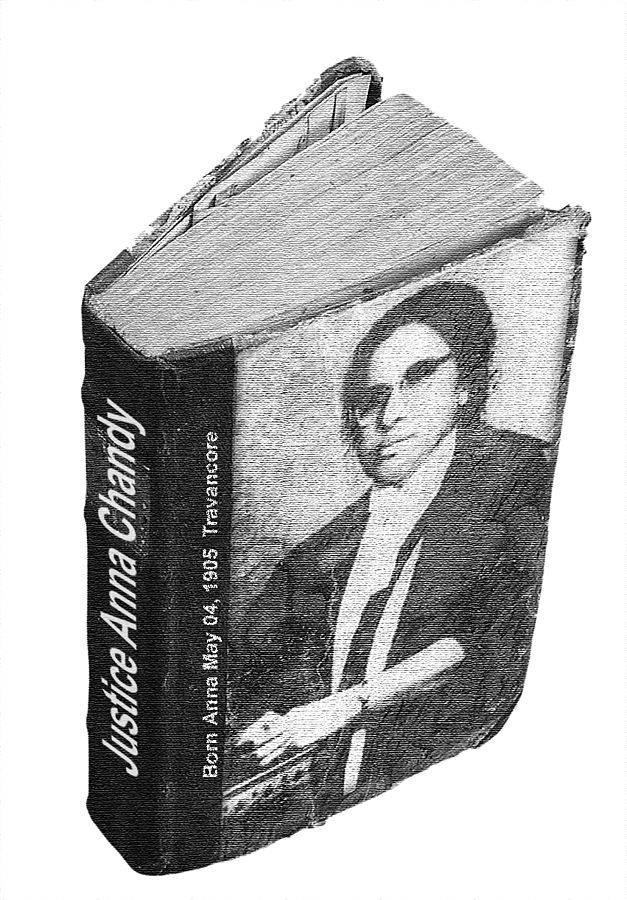
\includegraphics[width=0.5\textwidth,height=4cm]{Kulasthree_Chapter_three_pic07.jpg}
\end{center}

കേരളത്തിൽ നിയമബിരുദംനേടിയ ആദ്യത്ത വനിത, മുൻസിഫ് പദവിയിലെത്തിയ ആദ്യത്തെ സ്ത്രീ എന്നീ നിലകളിലാണ് അന്നാ ചാണ്ടി (1905-1996) ഇന്ന് അറിയപ്പെടുന്നത്. എന്നാൽ കേരളത്തിൽ സ്ത്രീകളുടെ അവകാശങ്ങൾക്കായി പൊരുതിയ ആദ്യകാല സ്ത്രീവാദി എന്ന അവരുടെ നില അത്ര പ്രസിദ്ധമല്ല. തിരുവനന്തപുരത്ത് അടിസ്ഥാനവിദ്യാഭ്യാസം പൂർത്തിയാക്കിയ അവർ 1926ൽ പ്രശസ്തമായ നിലയിൽ ബിരുദാനന്തരബിരുദം കരസ്ഥമാക്കി. പിന്നീട് നിയമപഠനത്തിനുശേഷം വക്കീൽ പദവിയിലേക്കു പ്രവേശിക്കുകയും ക്രിമിനൽവക്കീലായി പേരെടുക്കുകയും ചെയ്തു. ഒപ്പം, സ്ത്രീകളുടെ അവകാശങ്ങൾക്കായുള്ള പോരാട്ടങ്ങളുടെ മുന്നണിപ്പോരാളിയായി. തിരുവിതാംകൂറിലെ നിയമനിർമ്മാണസഭയായ ശ്രീമൂലംപ്രജാസഭയ്ക്കകത്തും പുറത്തും സ്ത്രീകളുടെ അവകാശങ്ങൾക്കായി ശബ്ദമുയർത്തി. 1930കളിൽ ശ്രീമതി എന്ന സ്ത്രീപക്ഷപ്രസിദ്ധീകരണത്തിന്റെ പ്രസാധകയായിരുന്നു. സ്വാതന്ത്ര്യാനന്തരകാലത്തിൽ ഔദ്യോഗികപദവിയിൽ മുന്നേറിയെങ്കിലും സ്ത്രീപക്ഷവക്താവ് എന്ന നിലയിൽ അവർ നിശബ്ദയായി. 1959ൽ ഹൈക്കോടതി ജഡ്ജിയായ അവർ 1967ൽ വിരമിച്ചു. ആത്മകഥയെഴുതി പ്രസിദ്ധീകരിച്ചെങ്കിലും അത്രയധികം ശ്രദ്ധിക്കപ്പെട്ടില്ല.
\end{tcolorbox}

\captionof{mybox}{കെ.ആർ. ഗൗരിയമ്മ}\label{ch3box4} % place the caption
\begin{tcolorbox}[%
 breakable, % make the box breakable
  arc=0mm, 
  left=1pt, right = 1pt, 
  boxrule=0mm,
  colback = {blue!10}, % since shadow-gray was not defined
] 
\begin{center}
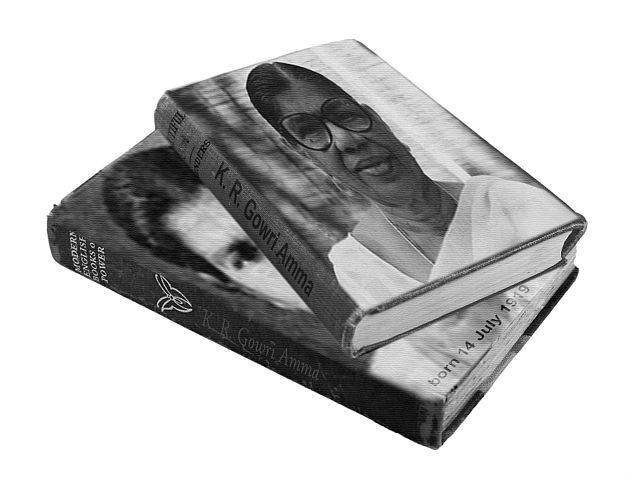
\includegraphics[width=0.5\textwidth,height=4cm]{Kulasthree_Chapter_three_pic08.jpg}
\end{center}
'ഒന്നാന്തരം പ്രക്ഷോഭകാരിണി, കഴിവുറ്റ ഭരണാധികാരിണി' - ഈ രണ്ട് അഭിനന്ദനങ്ങളും ഒരേസമയം ഏറ്റുവാങ്ങിയ മലയാളിസ്ത്രീയാണ് കെ.ആർ. ഗൗരിയമ്മ. 1987ൽ മുഖ്യമന്ത്രിപദത്തിനടുത്തെത്തിയെങ്കിലും ആ പദവി അവർക്കു ലഭിച്ചില്ലെന്നത് കേരളരാഷ്ട്രീയത്തിന്റെ ഉന്നതമേഖലകളിൽ സ്ത്രീകൾക്കു സ്ഥാനമില്ലെന്ന പരോക്ഷസന്ദേശംതന്നെയായിരുന്നു. 1919ൽ ജനിച്ച ഗൗരിയമ്മ ഈഴവസമുദായത്തിൽനിന്ന് നിയമബിരുദം നേടിയ ആദ്യത്തെ സ്ത്രീയായിരുന്നു. തെരഞ്ഞെടുപ്പുകളിൽ വിജയിക്കാൻ അസാമാന്യമായ കഴിവ് ആദ്യകാലങ്ങളിൽ അവർക്കുണ്ടായിരുന്നു. 1948ലെ തിരുവിതാംകൂറിലെ തെരഞ്ഞെടുപ്പിൽ (പ്രായപൂർത്തിവോട്ടവകാശം നടപ്പിലാക്കിയ ആദ്യത്തെ തെരഞ്ഞെടുപ്പിൽ) വെറും 28 വയസ്സുമാത്രം പ്രായമുണ്ടായിരുന്ന ഗൗരിയമ്മ ചേർത്തലയിൽ മുപ്പത്തിയഞ്ചുശതമാനം വോട്ട് നേടി - ഒരൊറ്റ കമ്യൂണിസ്റ്റ് സ്ഥാനാർത്ഥിപോലും ജയിക്കാത്ത തെരഞ്ഞെടുപ്പിൽ. അക്രമം പ്രചരിപ്പിച്ചുവെന്നാരോപിച്ച് സർക്കാർ അവരെ ജയിലിലടച്ചു. 1952ലെ തിരു-കൊച്ചി നിയമസഭാ തെരഞ്ഞെടുപ്പിൽ അരൂരിൽനിന്ന് അവർ വിജയിച്ചു. ആ സമയത്ത് അവർ ജയിലിലായിരുന്നു. 1977ൽ ഒഴിച്ച് എല്ലാ തെരെഞ്ഞെടുപ്പുകളിലും അവർ അവിടുന്ന് തെരഞ്ഞെടുക്കപ്പെട്ടു. 1987ൽ കേരളനിയമസഭയിലുണ്ടായിരുന്ന രണ്ടേരണ്ട് സി.പി.എം സ്ത്രീ അംഗങ്ങളിൽ ഒരാളായിരുന്നു. പിന്നീട്, സി.പി.എമ്മിനുള്ളിലെ അഭിപ്രായഭിന്നതകൾ രൂക്ഷമായതോടുകൂടി അവർ പാർട്ടി വിടുകയും സ്വന്തം പാർട്ടി രൂപീകരിക്കുകയും ചെയ്തു. അർഹിക്കുന്ന അംഗീകാരം ലഭിച്ചില്ലെങ്കിലും തൊണ്ണൂറാം വയസ്സിൽ, ഇന്നും ഗൗരിയമ്മ മലയാളിസ്ത്രീകളുടെ അഭിമാനമാണ്.

\end{tcolorbox}

\paragraph{}ഇന്ന് സ്ത്രീകളെ പൊതുരംഗത്തെത്തിക്കാൻ പല പരിപാടികളും ആവിഷ്ക്കരിക്കപ്പെടുന്നു. എങ്കിലും താഴേത്തട്ടിലും ചിലപ്പോൾ ഇടയിലുള്ള തട്ടുകളിലും സ്ത്രീകൾ എത്താറുണ്ടെങ്കിലും അധികാരരാഷ്ട്രീയത്തിന്റെ മുകൾത്തട്ടുകൾ പുരുഷന്മാരുടേതാണ്. കീഴ്ത്തട്ടുകളിൽപ്പോലും അധികാരത്തോടടുത്തുനിൽക്കുന്ന നിലകളെല്ലാം പുരുഷന്മാർക്കാണ്. പഞ്ചായത്തുഭരണത്തിൽ ഇപ്പോൾ സ്ത്രീകൾ പലയിടത്തും നന്നായി കഴിവു [ 68 ] തെളിയിക്കുന്നുണ്ടെങ്കിലും അതിലെത്രപേർക്ക് ഉന്നതരാഷ്ട്രീയത്തിലേക്ക് കടക്കാനായിട്ടുണ്ട്? പുരുഷന്മാരുടെ ഒപ്പം അവരുടെ രാഷ്ട്രീയ അടവുകൾ പയറ്റുന്ന കുറച്ചു സ്ത്രീകളുണ്ടെന്നത് വാസ്തവം തന്നെ. എന്നാലും അവരുടെ എണ്ണം വളരെ കുറവാണ്. അവർപോലും തരംകിട്ടുമ്പോൾ നല്ല പിള്ളകളായി സ്വയംചിത്രീകരിക്കാൻ ശ്രമിക്കാറുണ്ട്. അപ്പോൾ ചോദിച്ചുപോകും, രാജ്ഞി വെറും അമ്മറാണിമാത്രമാകുന്ന ആ കാലം യഥാർത്ഥത്തിൽ കടന്നുപൊയ്ക്കഴിഞ്ഞോ? സത്യത്തിൽ ഇന്നും നാം ആ കാലത്തിന്റെ പിടിയിൽത്തന്നെയല്ലേ?

\section{കൂടുതൽ ആലോചനയ്ക്ക്}

ഇവിടെ നാം ചർച്ചചെയ്തത് സ്ത്രീകളും ഭരണാധികാരവും തമ്മിലുള്ള ബന്ധത്തിന്റെ ചരിത്രമാണ്. ആ ചരിത്രം പരിശോധിക്കുമ്പോൾ കാണുന്ന കാര്യമിതാണ്: പെണ്ണുങ്ങൾക്ക് ഭരണാധികാരം വേണ്ട, അവർ കുടുംബിനികളും മാതാക്കന്മാരുമായിക്കൊള്ളട്ടെ എന്ന മനോഭാവം ഇവിടെ വിദേശഭരണത്തിനുമുമ്പുതന്നെ ആരംഭിക്കുന്നു. സ്ത്രീകളുടെ ചരിത്രത്തിന്റെ കാലഗണന മേലാളചരിത്രത്തിന്റേതിൽനിന്ന് വ്യത്യസ്തമായിരിക്കുമെന്ന് പറയാറുണ്ട്. ഉദാഹരണത്തിന് ലോകമഹായുദ്ധങ്ങളെക്കാൾ പടിഞ്ഞാറൻരാജ്യങ്ങളിലെ സ്ത്രീകളുടെ ജീവിതത്തെ കാര്യമായി മാറ്റിമറിച്ചത് ജനനനിയന്ത്രണമാർഗ്ഗങ്ങളുടെ കണ്ടുപിടിത്തമാണെന്ന് ചൂണ്ടിക്കാണിക്കപ്പെട്ടിട്ടുണ്ട്. ഇവിടെ ചർച്ചചെയ്തതിൽനിന്ന് ഇവിടത്തെ സ്ത്രീകളുടെ ചരിത്രത്തിനും സവിശേഷമായ ഒരു കാലഗണന ഉണ്ടെന്നല്ലേ തെളിയുന്നത്?

